\documentclass[twoside]{book}

% Packages required by doxygen
\usepackage{fixltx2e}
\usepackage{calc}
\usepackage{doxygen}
\usepackage[export]{adjustbox} % also loads graphicx
\usepackage{graphicx}
\usepackage[utf8]{inputenc}
\usepackage{makeidx}
\usepackage{multicol}
\usepackage{multirow}
\PassOptionsToPackage{warn}{textcomp}
\usepackage{textcomp}
\usepackage[nointegrals]{wasysym}
\usepackage[table]{xcolor}

% Font selection
\usepackage[T1]{fontenc}
\usepackage[scaled=.90]{helvet}
\usepackage{courier}
\usepackage{amssymb}
\usepackage{sectsty}
\renewcommand{\familydefault}{\sfdefault}
\allsectionsfont{%
  \fontseries{bc}\selectfont%
  \color{darkgray}%
}
\renewcommand{\DoxyLabelFont}{%
  \fontseries{bc}\selectfont%
  \color{darkgray}%
}
\newcommand{\+}{\discretionary{\mbox{\scriptsize$\hookleftarrow$}}{}{}}

% Page & text layout
\usepackage{geometry}
\geometry{%
  a4paper,%
  top=2.5cm,%
  bottom=2.5cm,%
  left=2.5cm,%
  right=2.5cm%
}
\tolerance=750
\hfuzz=15pt
\hbadness=750
\setlength{\emergencystretch}{15pt}
\setlength{\parindent}{0cm}
\setlength{\parskip}{3ex plus 2ex minus 2ex}
\makeatletter
\renewcommand{\paragraph}{%
  \@startsection{paragraph}{4}{0ex}{-1.0ex}{1.0ex}{%
    \normalfont\normalsize\bfseries\SS@parafont%
  }%
}
\renewcommand{\subparagraph}{%
  \@startsection{subparagraph}{5}{0ex}{-1.0ex}{1.0ex}{%
    \normalfont\normalsize\bfseries\SS@subparafont%
  }%
}
\makeatother

% Headers & footers
\usepackage{fancyhdr}
\pagestyle{fancyplain}
\fancyhead[LE]{\fancyplain{}{\bfseries\thepage}}
\fancyhead[CE]{\fancyplain{}{}}
\fancyhead[RE]{\fancyplain{}{\bfseries\leftmark}}
\fancyhead[LO]{\fancyplain{}{\bfseries\rightmark}}
\fancyhead[CO]{\fancyplain{}{}}
\fancyhead[RO]{\fancyplain{}{\bfseries\thepage}}
\fancyfoot[LE]{\fancyplain{}{}}
\fancyfoot[CE]{\fancyplain{}{}}
\fancyfoot[RE]{\fancyplain{}{\bfseries\scriptsize Generated by Doxygen }}
\fancyfoot[LO]{\fancyplain{}{\bfseries\scriptsize Generated by Doxygen }}
\fancyfoot[CO]{\fancyplain{}{}}
\fancyfoot[RO]{\fancyplain{}{}}
\renewcommand{\footrulewidth}{0.4pt}
\renewcommand{\chaptermark}[1]{%
  \markboth{#1}{}%
}
\renewcommand{\sectionmark}[1]{%
  \markright{\thesection\ #1}%
}

% Indices & bibliography
\usepackage{natbib}
\usepackage[titles]{tocloft}
\setcounter{tocdepth}{3}
\setcounter{secnumdepth}{5}
\makeindex

% Hyperlinks (required, but should be loaded last)
\usepackage{ifpdf}
\ifpdf
  \usepackage[pdftex,pagebackref=true]{hyperref}
\else
  \usepackage[ps2pdf,pagebackref=true]{hyperref}
\fi
\hypersetup{%
  colorlinks=true,%
  linkcolor=blue,%
  citecolor=blue,%
  unicode%
}

% Custom commands
\newcommand{\clearemptydoublepage}{%
  \newpage{\pagestyle{empty}\cleardoublepage}%
}

\usepackage{caption}
\captionsetup{labelsep=space,justification=centering,font={bf},singlelinecheck=off,skip=4pt,position=top}

%===== C O N T E N T S =====

\begin{document}

% Titlepage & ToC
\hypersetup{pageanchor=false,
             bookmarksnumbered=true,
             pdfencoding=unicode
            }
\pagenumbering{alph}
\begin{titlepage}
\vspace*{7cm}
\begin{center}%
{\Large Ci\+A402\+Device }\\
\vspace*{1cm}
{\large Generated by Doxygen 1.8.13}\\
\end{center}
\end{titlepage}
\clearemptydoublepage
\pagenumbering{roman}
\tableofcontents
\clearemptydoublepage
\pagenumbering{arabic}
\hypersetup{pageanchor=true}

%--- Begin generated contents ---
\chapter{Ci\+A402\+Device}
\label{md_README}
\Hypertarget{md_README}
Library under CiA 402 standard for device control 
\chapter{Hierarchical Index}
\section{Class Hierarchy}
This inheritance list is sorted roughly, but not completely, alphabetically\+:\begin{DoxyCompactList}
\item \contentsline{section}{can\+\_\+filter}{\pageref{structcan__filter}}{}
\item \contentsline{section}{can\+\_\+msg}{\pageref{structcan__msg}}{}
\item \contentsline{section}{Ci\+A301\+Comm\+Port}{\pageref{classCiA301CommPort}}{}
\begin{DoxyCompactList}
\item \contentsline{section}{Ci\+A402\+Device}{\pageref{classCiA402Device}}{}
\end{DoxyCompactList}
\item \contentsline{section}{Ci\+A402\+Device\+I\+Canbus}{\pageref{classCiA402DeviceICanbus}}{}
\item \contentsline{section}{co\+\_\+msg}{\pageref{structco__msg}}{}
\item \contentsline{section}{Device\+Chain}{\pageref{classDeviceChain}}{}
\item \contentsline{section}{err\+\_\+stat}{\pageref{structerr__stat}}{}
\item \contentsline{section}{Port\+Base}{\pageref{classPortBase}}{}
\begin{DoxyCompactList}
\item \contentsline{section}{Can\+Bus\+Port}{\pageref{classCanBusPort}}{}
\item \contentsline{section}{Socket\+Can\+Port}{\pageref{classSocketCanPort}}{}
\item \contentsline{section}{Test\+Port}{\pageref{classTestPort}}{}
\end{DoxyCompactList}
\end{DoxyCompactList}

\chapter{Class Index}
\section{Class List}
Here are the classes, structs, unions and interfaces with brief descriptions\+:\begin{DoxyCompactList}
\item\contentsline{section}{\hyperlink{structcan__filter}{can\+\_\+filter} }{\pageref{structcan__filter}}{}
\item\contentsline{section}{\hyperlink{structcan__msg}{can\+\_\+msg} }{\pageref{structcan__msg}}{}
\item\contentsline{section}{\hyperlink{classCanBusPort}{Can\+Bus\+Port} }{\pageref{classCanBusPort}}{}
\item\contentsline{section}{\hyperlink{classCiA301CommPort}{Ci\+A301\+Comm\+Port} }{\pageref{classCiA301CommPort}}{}
\item\contentsline{section}{\hyperlink{classCiA402Device}{Ci\+A402\+Device} }{\pageref{classCiA402Device}}{}
\item\contentsline{section}{\hyperlink{classCiA402DeviceICanbus}{Ci\+A402\+Device\+I\+Canbus} }{\pageref{classCiA402DeviceICanbus}}{}
\item\contentsline{section}{\hyperlink{structco__msg}{co\+\_\+msg} }{\pageref{structco__msg}}{}
\item\contentsline{section}{\hyperlink{classDeviceChain}{Device\+Chain} }{\pageref{classDeviceChain}}{}
\item\contentsline{section}{\hyperlink{structerr__stat}{err\+\_\+stat} }{\pageref{structerr__stat}}{}
\item\contentsline{section}{\hyperlink{classPortBase}{Port\+Base} }{\pageref{classPortBase}}{}
\item\contentsline{section}{\hyperlink{classSocketCanPort}{Socket\+Can\+Port} }{\pageref{classSocketCanPort}}{}
\item\contentsline{section}{\hyperlink{classTestPort}{Test\+Port} }{\pageref{classTestPort}}{}
\end{DoxyCompactList}

\chapter{Class Documentation}
\hypertarget{structcan__filter}{}\section{can\+\_\+filter Struct Reference}
\label{structcan__filter}\index{can\+\_\+filter@{can\+\_\+filter}}
\subsection*{Public Attributes}
\begin{DoxyCompactItemize}
\item 
\mbox{\Hypertarget{structcan__filter_a796cdd0845b3b22c44028a898938d3e0}\label{structcan__filter_a796cdd0845b3b22c44028a898938d3e0}} 
int {\bfseries type}
\item 
\mbox{\Hypertarget{structcan__filter_a4831e5deb6d6475d8cad3ceae529c51f}\label{structcan__filter_a4831e5deb6d6475d8cad3ceae529c51f}} 
\begin{tabbing}
xx\=xx\=xx\=xx\=xx\=xx\=xx\=xx\=xx\=\kill
union \{\\
\>uint32\_t {\bfseries mask}\\
\>uint32\_t {\bfseries upper}\\
\}; \\

\end{tabbing}\item 
\mbox{\Hypertarget{structcan__filter_afbb39bd7340f5fa3ce79d138919840d8}\label{structcan__filter_afbb39bd7340f5fa3ce79d138919840d8}} 
\begin{tabbing}
xx\=xx\=xx\=xx\=xx\=xx\=xx\=xx\=xx\=\kill
union \{\\
\>uint32\_t {\bfseries code}\\
\>uint32\_t {\bfseries lower}\\
\}; \\

\end{tabbing}\end{DoxyCompactItemize}


The documentation for this struct was generated from the following file\+:\begin{DoxyCompactItemize}
\item 
hico\+\_\+api.\+h\end{DoxyCompactItemize}

\hypertarget{structcan__msg}{}\section{can\+\_\+msg Struct Reference}
\label{structcan__msg}\index{can\+\_\+msg@{can\+\_\+msg}}
\subsection*{Public Attributes}
\begin{DoxyCompactItemize}
\item 
\mbox{\Hypertarget{structcan__msg_a233f7f010cc90ec3d453bcb75d66c14e}\label{structcan__msg_a233f7f010cc90ec3d453bcb75d66c14e}} 
\begin{tabbing}
xx\=xx\=xx\=xx\=xx\=xx\=xx\=xx\=xx\=\kill
union \{\\
\>uint16\_t {\bfseries fi}\\
\} {\bfseries PACKED}\\

\end{tabbing}\item 
\mbox{\Hypertarget{structcan__msg_a157aaad2daf039f59606522c6a51663a}\label{structcan__msg_a157aaad2daf039f59606522c6a51663a}} 
uint32\+\_\+t {\bfseries ts}
\item 
\mbox{\Hypertarget{structcan__msg_a9a5f820883d3dfe1f0c6bc33c3f95989}\label{structcan__msg_a9a5f820883d3dfe1f0c6bc33c3f95989}} 
uint32\+\_\+t {\bfseries id}
\item 
\mbox{\Hypertarget{structcan__msg_ac0dab268ebadaa9521b4d535c03f13d8}\label{structcan__msg_ac0dab268ebadaa9521b4d535c03f13d8}} 
uint8\+\_\+t {\bfseries data} \mbox{[}8\mbox{]}
\item 
\mbox{\Hypertarget{structcan__msg_a11a48cac095afd9250fe22fa37929aec}\label{structcan__msg_a11a48cac095afd9250fe22fa37929aec}} 
\begin{tabbing}
xx\=xx\=xx\=xx\=xx\=xx\=xx\=xx\=xx\=\kill
union \{\\
\>uint16\_t {\bfseries fi}\\
\} {\bfseries PACKED}\\

\end{tabbing}\end{DoxyCompactItemize}


The documentation for this struct was generated from the following files\+:\begin{DoxyCompactItemize}
\item 
candatatypes.\+h\item 
hico\+\_\+api.\+h\end{DoxyCompactItemize}

\hypertarget{classCanBusPort}{}\section{Can\+Bus\+Port Class Reference}
\label{classCanBusPort}\index{Can\+Bus\+Port@{Can\+Bus\+Port}}


Inheritance diagram for Can\+Bus\+Port\+:
\nopagebreak
\begin{figure}[H]
\begin{center}
\leavevmode
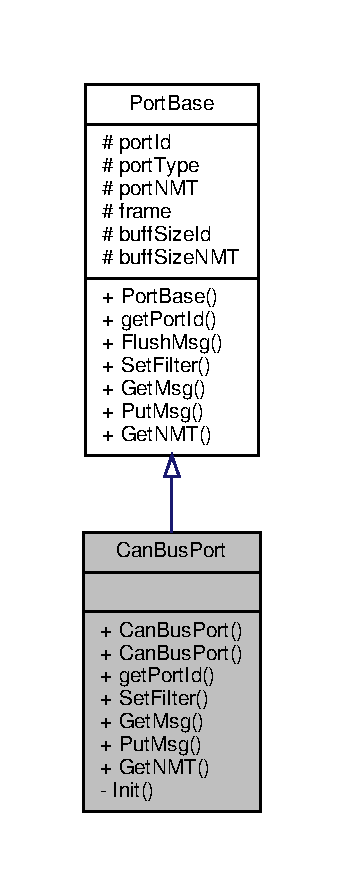
\includegraphics[width=150pt]{classCanBusPort__inherit__graph}
\end{center}
\end{figure}


Collaboration diagram for Can\+Bus\+Port\+:
\nopagebreak
\begin{figure}[H]
\begin{center}
\leavevmode
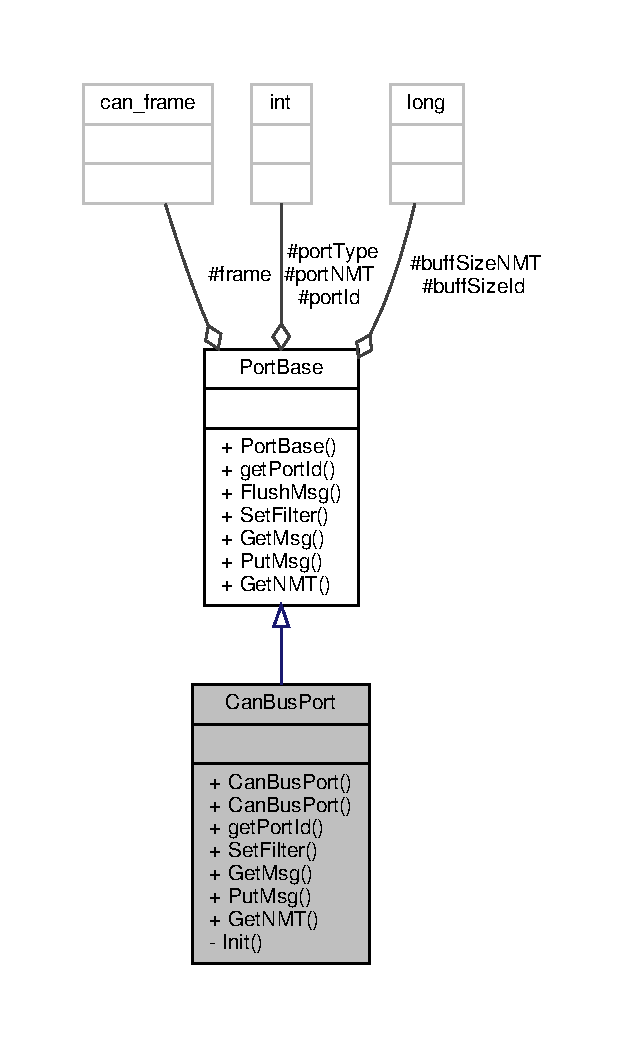
\includegraphics[width=150pt]{classCanBusPort__coll__graph}
\end{center}
\end{figure}
\subsection*{Public Member Functions}
\begin{DoxyCompactItemize}
\item 
\mbox{\Hypertarget{classCanBusPort_a4ccb8d39da6185bfe5c1dee38db51987}\label{classCanBusPort_a4ccb8d39da6185bfe5c1dee38db51987}} 
\hyperlink{classCanBusPort_a4ccb8d39da6185bfe5c1dee38db51987}{Can\+Bus\+Port} ()
\begin{DoxyCompactList}\small\item\em \hyperlink{classCanBusPort}{Can\+Bus\+Port}\+: Empty constructor. Initialize default port \char`\"{}/dev/can0\char`\"{}. \end{DoxyCompactList}\item 
\hyperlink{classCanBusPort_ad4649a2da594bbffc267483646fb1405}{Can\+Bus\+Port} (string can\+Port)
\begin{DoxyCompactList}\small\item\em \hyperlink{classCanBusPort}{Can\+Bus\+Port}\+: Initialization of one port given a device name. \end{DoxyCompactList}\item 
\mbox{\Hypertarget{classCanBusPort_a7c6b733c5834d4ab3e1906d847a2234a}\label{classCanBusPort_a7c6b733c5834d4ab3e1906d847a2234a}} 
int {\bfseries get\+Port\+Id} ()
\item 
\mbox{\Hypertarget{classCanBusPort_af09c794e3af86e89c8a511535f856dc9}\label{classCanBusPort_af09c794e3af86e89c8a511535f856dc9}} 
long {\bfseries Set\+Filter} (uint32\+\_\+t can\+Id, uint32\+\_\+t mask)
\item 
\mbox{\Hypertarget{classCanBusPort_a13d6b06d93debc20b2f49aa8e7139988}\label{classCanBusPort_a13d6b06d93debc20b2f49aa8e7139988}} 
long {\bfseries Get\+Msg} (uint32\+\_\+t \&can\+Id, uint8\+\_\+t $\ast$data, uint8\+\_\+t size)
\item 
\mbox{\Hypertarget{classCanBusPort_a2bb802ad7a14e260f0f51b79d4c53c43}\label{classCanBusPort_a2bb802ad7a14e260f0f51b79d4c53c43}} 
long {\bfseries Put\+Msg} (const uint32\+\_\+t \&can\+Id, uint8\+\_\+t $\ast$const data, const uint8\+\_\+t size)
\item 
\mbox{\Hypertarget{classCanBusPort_a41242dc7980ca398e4770813e50ef32b}\label{classCanBusPort_a41242dc7980ca398e4770813e50ef32b}} 
long {\bfseries Get\+N\+MT} (uint8\+\_\+t $\ast$const data, uint8\+\_\+t \&size)
\end{DoxyCompactItemize}
\subsection*{Additional Inherited Members}


\subsection{Constructor \& Destructor Documentation}
\mbox{\Hypertarget{classCanBusPort_ad4649a2da594bbffc267483646fb1405}\label{classCanBusPort_ad4649a2da594bbffc267483646fb1405}} 
\index{Can\+Bus\+Port@{Can\+Bus\+Port}!Can\+Bus\+Port@{Can\+Bus\+Port}}
\index{Can\+Bus\+Port@{Can\+Bus\+Port}!Can\+Bus\+Port@{Can\+Bus\+Port}}
\subsubsection{\texorpdfstring{Can\+Bus\+Port()}{CanBusPort()}}
{\footnotesize\ttfamily Can\+Bus\+Port\+::\+Can\+Bus\+Port (\begin{DoxyParamCaption}\item[{string}]{can\+Port }\end{DoxyParamCaption})}



\hyperlink{classCanBusPort}{Can\+Bus\+Port}\+: Initialization of one port given a device name. 


\begin{DoxyParams}{Parameters}
{\em can\+Port} & String with the name of system device. \\
\hline
\end{DoxyParams}


The documentation for this class was generated from the following files\+:\begin{DoxyCompactItemize}
\item 
Can\+Bus\+Port.\+h\item 
Can\+Bus\+Port.\+cpp\end{DoxyCompactItemize}

\hypertarget{classCiA301CommPort}{}\section{Ci\+A301\+Comm\+Port Class Reference}
\label{classCiA301CommPort}\index{Ci\+A301\+Comm\+Port@{Ci\+A301\+Comm\+Port}}


{\ttfamily \#include $<$Ci\+A301\+Comm\+Port.\+h$>$}



Inheritance diagram for Ci\+A301\+Comm\+Port\+:\nopagebreak
\begin{figure}[H]
\begin{center}
\leavevmode
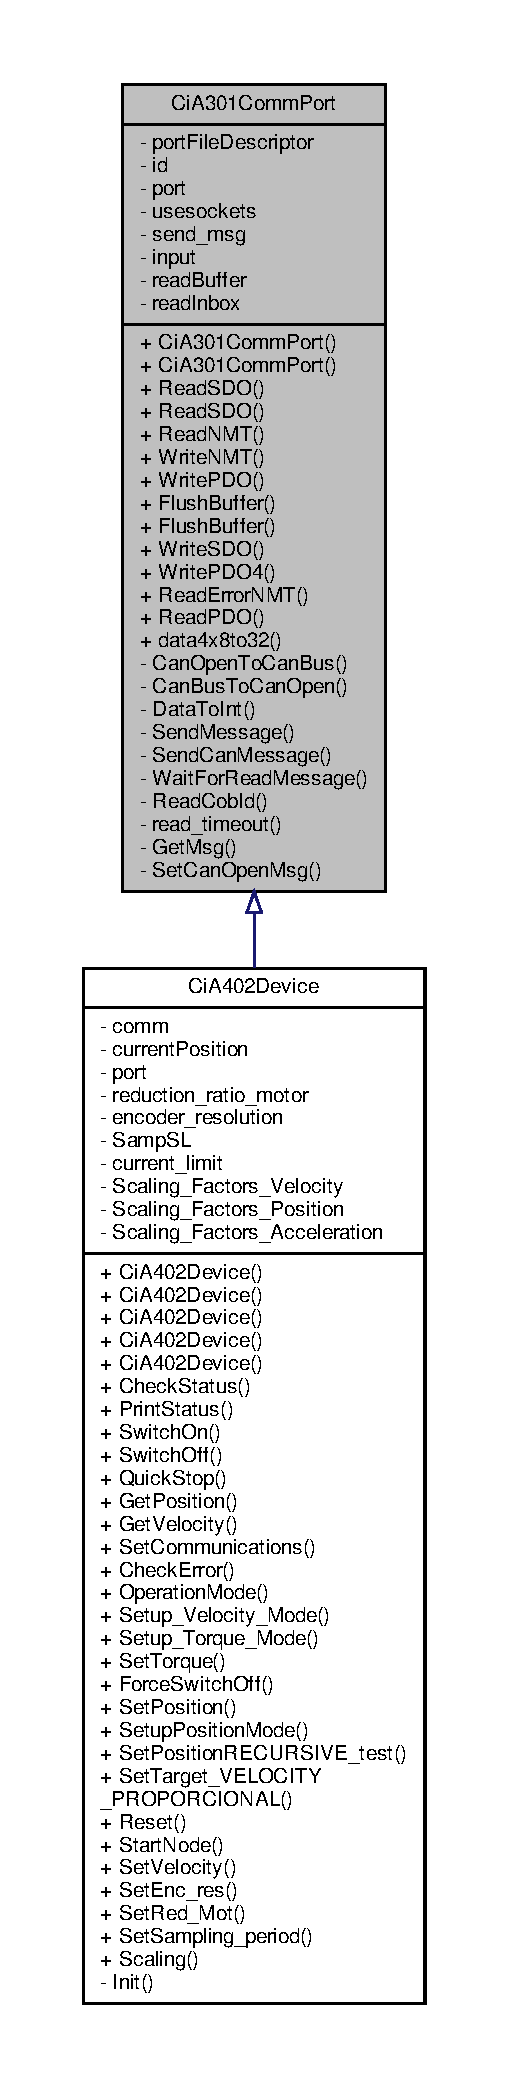
\includegraphics[height=550pt]{classCiA301CommPort__inherit__graph}
\end{center}
\end{figure}


Collaboration diagram for Ci\+A301\+Comm\+Port\+:\nopagebreak
\begin{figure}[H]
\begin{center}
\leavevmode
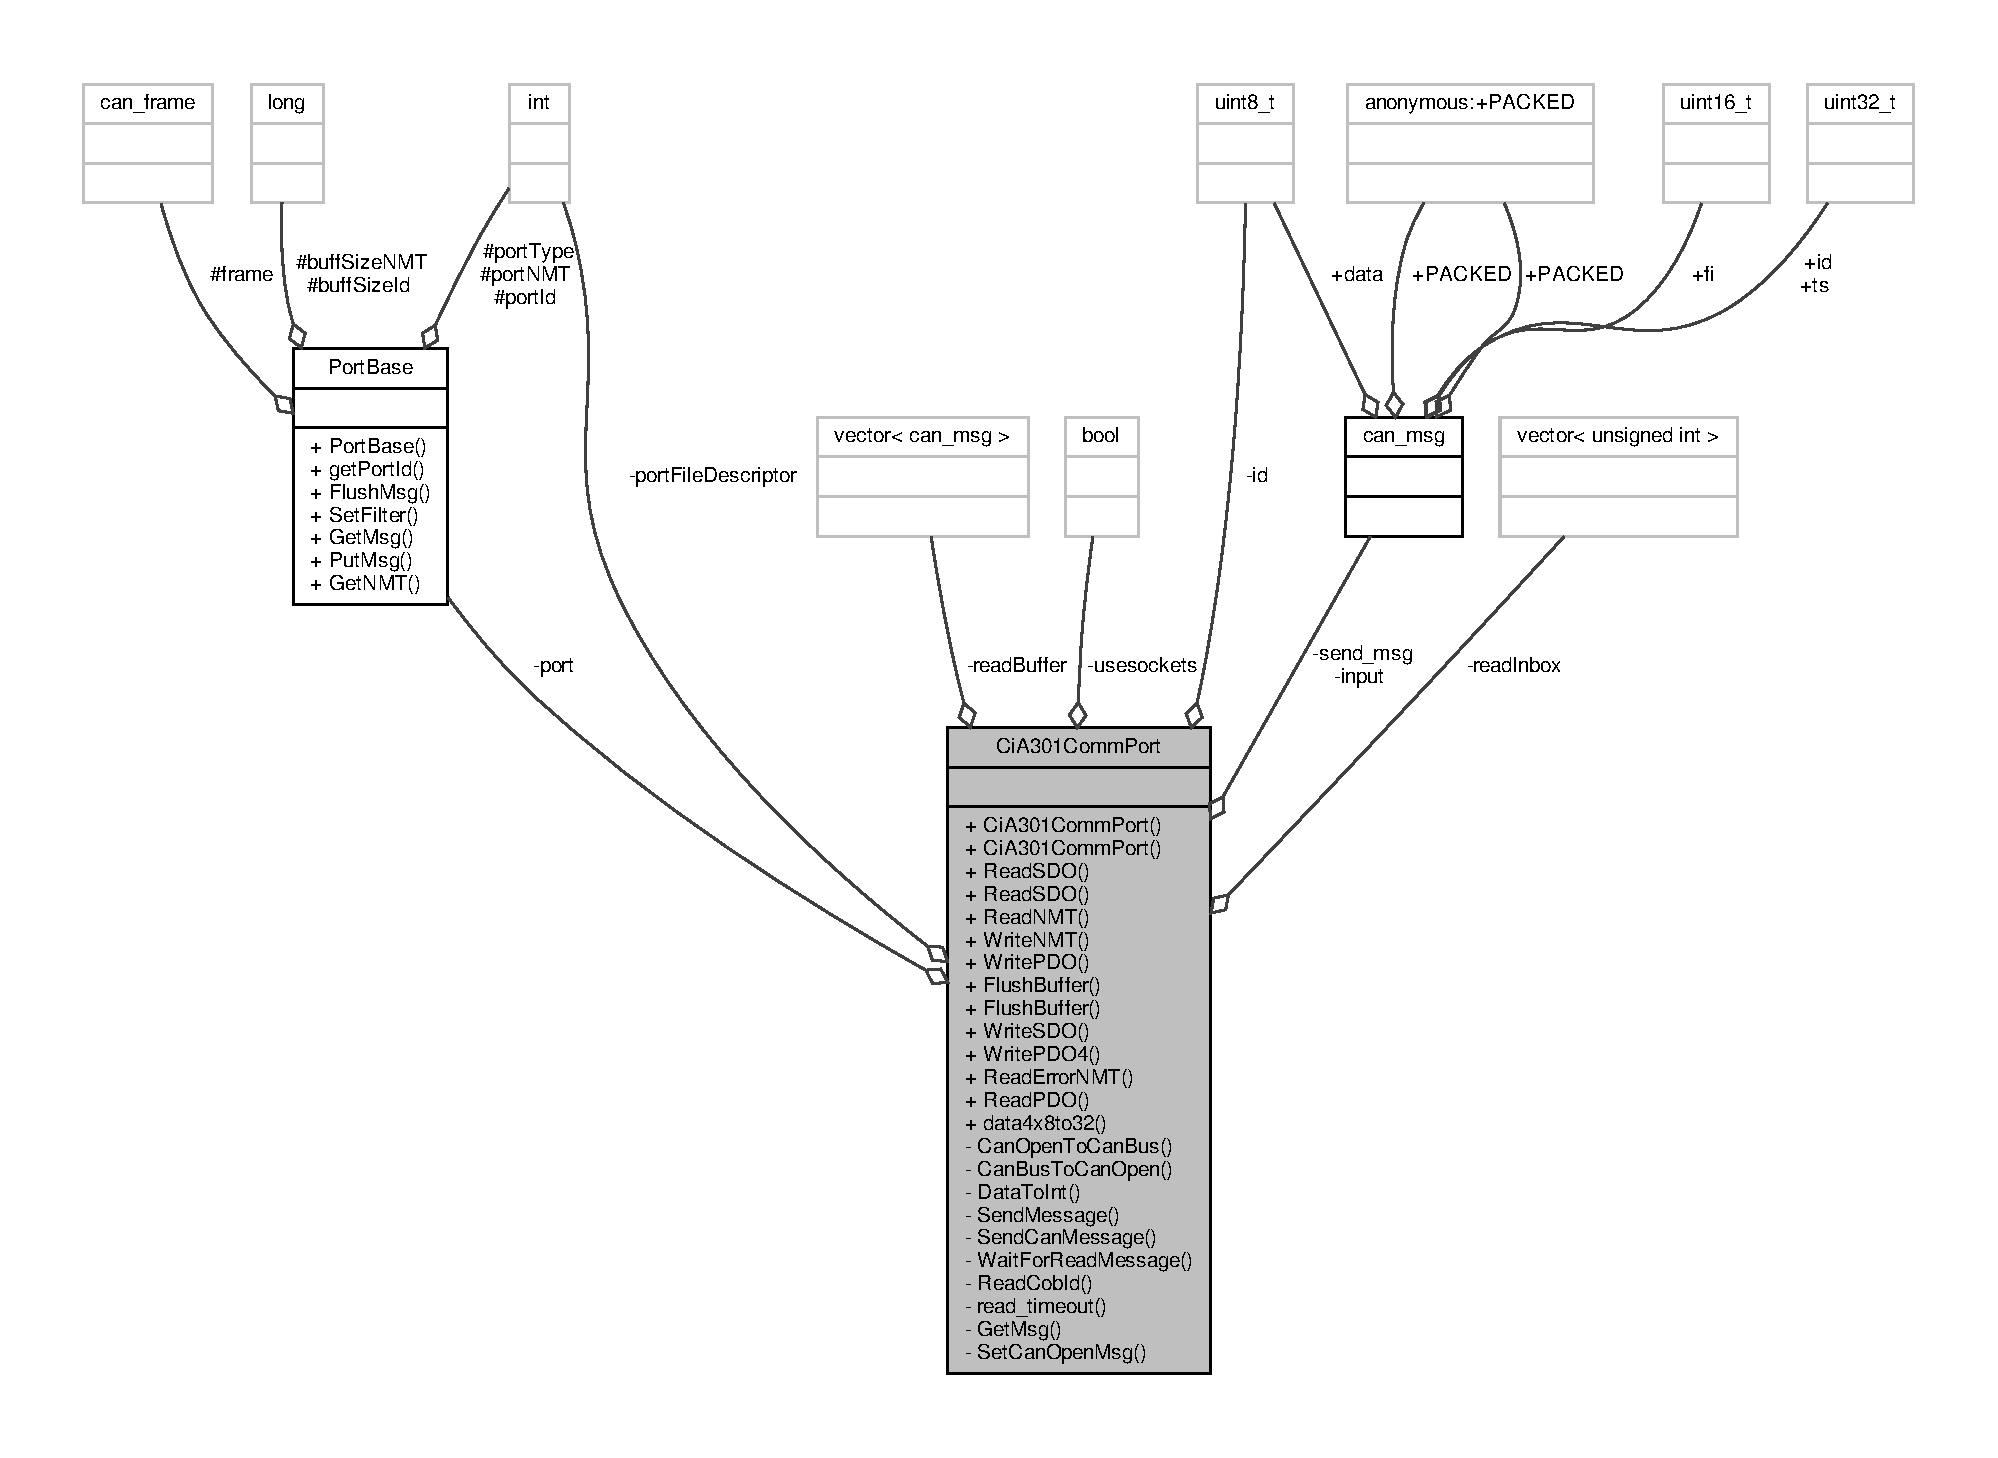
\includegraphics[width=350pt]{classCiA301CommPort__coll__graph}
\end{center}
\end{figure}
\subsection*{Public Member Functions}
\begin{DoxyCompactItemize}
\item 
\hyperlink{classCiA301CommPort_aae705cb5c6a405ef74a10e5220d0b08f}{Ci\+A301\+Comm\+Port} (int new\+Port\+File\+Descriptor, uint8\+\_\+t new\+\_\+id)
\item 
\hyperlink{classCiA301CommPort_a1e05c4b292cfee36ff9eeddb2c8eb4c0}{Ci\+A301\+Comm\+Port} (\hyperlink{classPortBase}{Port\+Base} $\ast$new\+\_\+port, uint8\+\_\+t new\+\_\+id)
\item 
long \hyperlink{classCiA301CommPort_a0fd0920052684589bc37bb898dcdd758}{Read\+S\+DO} (vector$<$ uint8\+\_\+t $>$ address, int subindex)
\item 
long \hyperlink{classCiA301CommPort_a3f74ce5899b30731322dabd352ccdc55}{Read\+S\+DO} (const vector$<$ uint8\+\_\+t $>$ \&address)
\begin{DoxyCompactList}\small\item\em \hyperlink{classCiA301CommPort_a0fd0920052684589bc37bb898dcdd758}{Ci\+A301\+Comm\+Port\+::\+Read\+S\+DO} Waits until expected. \end{DoxyCompactList}\item 
long \hyperlink{classCiA301CommPort_a02df85ed5140d0d7a57fe0d2f6e47ea1}{Read\+N\+MT} (const vector$<$ uint8\+\_\+t $>$ \&nmt\+Code)
\item 
long \hyperlink{classCiA301CommPort_a09feb3f78831c9fbb683a85cc3bc4562}{Write\+N\+MT} (const vector$<$ uint8\+\_\+t $>$ \&nmt\+Command)
\begin{DoxyCompactList}\small\item\em Write\+N\+MT This function sends N\+MT message from node to Can\+Bus. \end{DoxyCompactList}\item 
long \hyperlink{classCiA301CommPort_a56d2c604b11363e6b287f59b68a546bd}{Write\+P\+DO} (const vector$<$ uint8\+\_\+t $>$ \&command)
\begin{DoxyCompactList}\small\item\em Write\+P\+DO This function sends P\+DO message to a node (the mode id is configured on constructor). \end{DoxyCompactList}\item 
long \hyperlink{classCiA301CommPort_a067cddaf01932fa6fa27255c61b08190}{Flush\+Buffer} ()
\item 
long \hyperlink{classCiA301CommPort_ab29e221039a2d21d1446edb09b91864e}{Flush\+Buffer} (int msgs)
\begin{DoxyCompactList}\small\item\em Flush\+Buffer Removes the msgs number of can frames from buffer. \end{DoxyCompactList}\item 
long \hyperlink{classCiA301CommPort_a4d97c27423b2323f8475f6e5c2f91575}{Write\+S\+DO} (const vector$<$ uint8\+\_\+t $>$ \&address, const vector$<$ uint8\+\_\+t $>$ \&value)
\begin{DoxyCompactList}\small\item\em Write\+S\+DO Writes 4 byte value to specific address on device. This function sends S\+DO message requesting write on the object dictionary address. Also block and wait for the S\+DO msg for write ack, and returns negative if error. As it reads the ack S\+DO message, the buffer should be same size after this function returns. \end{DoxyCompactList}\item 
long \hyperlink{classCiA301CommPort_a1faf4f37530e0dd0ae4600cfb0b1d742}{Write\+P\+D\+O4} (const vector$<$ uint8\+\_\+t $>$ \&command)
\item 
long \hyperlink{classCiA301CommPort_a46534ff9e7e2a05a0b4913e4331710e5}{Read\+Error\+N\+MT} ()
\item 
long \hyperlink{classCiA301CommPort_a827f3e594b9f1e57a7b7ccb8a278404a}{Read\+P\+DO} (long number)
\end{DoxyCompactItemize}
\subsection*{Private Member Functions}
\begin{DoxyCompactItemize}
\item 
long \hyperlink{classCiA301CommPort_a26346f83700bc8403a315be01c6508e0}{Can\+Open\+To\+Can\+Bus} (const \hyperlink{structco__msg}{co\+\_\+msg} \&\hyperlink{classCiA301CommPort_ae0f955c7141e2067307cea0b48e111d4}{input}, \hyperlink{structcan__msg}{can\+\_\+msg} \&output)
\item 
long \hyperlink{classCiA301CommPort_aa16887712ea9cad534aacd4851f9190d}{Can\+Bus\+To\+Can\+Open} (const \hyperlink{structcan__msg}{can\+\_\+msg} \&\hyperlink{classCiA301CommPort_ae0f955c7141e2067307cea0b48e111d4}{input}, \hyperlink{structco__msg}{co\+\_\+msg} \&output)
\item 
uint32\+\_\+t \hyperlink{classCiA301CommPort_a77ec43d792a81489e221c3990225e57b}{data4x8to32} (const uint8\+\_\+t $\ast$in)
\item 
uint32\+\_\+t \hyperlink{classCiA301CommPort_a2bbd06fc6ae74727cef148911e433495}{Data\+To\+Int} (const uint8\+\_\+t $\ast$in, const uint8\+\_\+t size)
\item 
int \hyperlink{classCiA301CommPort_aeae04455e1e1a1ca1beed9478372c031}{Send\+Message} (\hyperlink{structco__msg}{co\+\_\+msg} \hyperlink{classCiA301CommPort_ae0f955c7141e2067307cea0b48e111d4}{input})
\item 
int \hyperlink{classCiA301CommPort_a700a04da67928ca50744617ece28cde5}{Send\+Can\+Message} (\hyperlink{structcan__msg}{can\+\_\+msg} \&\hyperlink{classCiA301CommPort_ae0f955c7141e2067307cea0b48e111d4}{input})
\item 
int \hyperlink{classCiA301CommPort_a02ba7069a0497e3497f3dfaec2879b54}{Wait\+For\+Read\+Message} (\hyperlink{structco__msg}{co\+\_\+msg} \&output, unsigned int can\+Index)
\item 
int \hyperlink{classCiA301CommPort_a408f53d13935a1916ca6f21d08ae135e}{Read\+Cob\+Id} (uint16\+\_\+t expected\+\_\+cobid, \hyperlink{structco__msg}{co\+\_\+msg} \&output)
\begin{DoxyCompactList}\small\item\em Ci\+A301\+Comm\+Port\+::\+Wait\+For\+Answer Read the port until expected canopen answer shows up in the port reads. \end{DoxyCompactList}\item 
int \hyperlink{classCiA301CommPort_ae62c2389b38a0e217aff7ca17a3d87b6}{read\+\_\+timeout} (int fd, \hyperlink{structcan__msg}{can\+\_\+msg} $\ast$buf, unsigned int timeout)
\item 
long \hyperlink{classCiA301CommPort_a645450ca09e07ea6da339923ceeec934}{Get\+Msg} (\hyperlink{structcan__msg}{can\+\_\+msg} \&msg)
\item 
\hyperlink{structco__msg}{co\+\_\+msg} \hyperlink{classCiA301CommPort_a2c197480112989df6bdb9ea89a649636}{Set\+Can\+Open\+Msg} (unsigned short id\+\_\+co, unsigned short rtr, vector$<$ uint8\+\_\+t $>$ co\+Data\+Frame)
\begin{DoxyCompactList}\small\item\em \hyperlink{classCiA402DeviceICanbus_aa439b9175f5879282058a3f4c2edb45d}{Ci\+A402\+Device\+I\+Canbus\+::\+Set\+Can\+Open\+Msg} \+: Constructs canopen message from parameters. \end{DoxyCompactList}\end{DoxyCompactItemize}
\subsection*{Private Attributes}
\begin{DoxyCompactItemize}
\item 
int \hyperlink{classCiA301CommPort_adc50c8d333b18fcb1b5c61ca69ea05c6}{port\+File\+Descriptor}
\item 
uint8\+\_\+t \hyperlink{classCiA301CommPort_a1ae075d22fc854da21a6e691bb029fc0}{id}
\item 
\hyperlink{classPortBase}{Port\+Base} $\ast$ \hyperlink{classCiA301CommPort_a6b8366387075c99ee980d2ca79c7b7fc}{port}
\item 
bool \hyperlink{classCiA301CommPort_a579e0de814111bde3bbe18cceb76ce64}{usesockets}
\item 
\hyperlink{structcan__msg}{can\+\_\+msg} \hyperlink{classCiA301CommPort_ade81ac897a5d851d946dd7a18245b75d}{send\+\_\+msg}
\item 
\hyperlink{structcan__msg}{can\+\_\+msg} \hyperlink{classCiA301CommPort_ae0f955c7141e2067307cea0b48e111d4}{input}
\item 
vector$<$ \hyperlink{structcan__msg}{can\+\_\+msg} $>$ \hyperlink{classCiA301CommPort_a8b904f3591ecfb99fd82271343727215}{read\+Buffer}
\item 
vector$<$ unsigned int $>$ \hyperlink{classCiA301CommPort_a41b2fcb24a27e5280417db03d8cdb399}{read\+Inbox}
\end{DoxyCompactItemize}


\subsection{Constructor \& Destructor Documentation}
\mbox{\Hypertarget{classCiA301CommPort_aae705cb5c6a405ef74a10e5220d0b08f}\label{classCiA301CommPort_aae705cb5c6a405ef74a10e5220d0b08f}} 
\index{Ci\+A301\+Comm\+Port@{Ci\+A301\+Comm\+Port}!Ci\+A301\+Comm\+Port@{Ci\+A301\+Comm\+Port}}
\index{Ci\+A301\+Comm\+Port@{Ci\+A301\+Comm\+Port}!Ci\+A301\+Comm\+Port@{Ci\+A301\+Comm\+Port}}
\subsubsection{\texorpdfstring{Ci\+A301\+Comm\+Port()}{CiA301CommPort()}\hspace{0.1cm}{\footnotesize\ttfamily [1/2]}}
{\footnotesize\ttfamily Ci\+A301\+Comm\+Port\+::\+Ci\+A301\+Comm\+Port (\begin{DoxyParamCaption}\item[{int}]{new\+Port\+File\+Descriptor,  }\item[{uint8\+\_\+t}]{new\+\_\+id }\end{DoxyParamCaption})}

\mbox{\Hypertarget{classCiA301CommPort_a1e05c4b292cfee36ff9eeddb2c8eb4c0}\label{classCiA301CommPort_a1e05c4b292cfee36ff9eeddb2c8eb4c0}} 
\index{Ci\+A301\+Comm\+Port@{Ci\+A301\+Comm\+Port}!Ci\+A301\+Comm\+Port@{Ci\+A301\+Comm\+Port}}
\index{Ci\+A301\+Comm\+Port@{Ci\+A301\+Comm\+Port}!Ci\+A301\+Comm\+Port@{Ci\+A301\+Comm\+Port}}
\subsubsection{\texorpdfstring{Ci\+A301\+Comm\+Port()}{CiA301CommPort()}\hspace{0.1cm}{\footnotesize\ttfamily [2/2]}}
{\footnotesize\ttfamily Ci\+A301\+Comm\+Port\+::\+Ci\+A301\+Comm\+Port (\begin{DoxyParamCaption}\item[{\hyperlink{classPortBase}{Port\+Base} $\ast$}]{new\+\_\+port,  }\item[{uint8\+\_\+t}]{new\+\_\+id }\end{DoxyParamCaption})}



\subsection{Member Function Documentation}
\mbox{\Hypertarget{classCiA301CommPort_aa16887712ea9cad534aacd4851f9190d}\label{classCiA301CommPort_aa16887712ea9cad534aacd4851f9190d}} 
\index{Ci\+A301\+Comm\+Port@{Ci\+A301\+Comm\+Port}!Can\+Bus\+To\+Can\+Open@{Can\+Bus\+To\+Can\+Open}}
\index{Can\+Bus\+To\+Can\+Open@{Can\+Bus\+To\+Can\+Open}!Ci\+A301\+Comm\+Port@{Ci\+A301\+Comm\+Port}}
\subsubsection{\texorpdfstring{Can\+Bus\+To\+Can\+Open()}{CanBusToCanOpen()}}
{\footnotesize\ttfamily long Ci\+A301\+Comm\+Port\+::\+Can\+Bus\+To\+Can\+Open (\begin{DoxyParamCaption}\item[{const \hyperlink{structcan__msg}{can\+\_\+msg} \&}]{input,  }\item[{\hyperlink{structco__msg}{co\+\_\+msg} \&}]{output }\end{DoxyParamCaption})\hspace{0.3cm}{\ttfamily [private]}}

\mbox{\Hypertarget{classCiA301CommPort_a26346f83700bc8403a315be01c6508e0}\label{classCiA301CommPort_a26346f83700bc8403a315be01c6508e0}} 
\index{Ci\+A301\+Comm\+Port@{Ci\+A301\+Comm\+Port}!Can\+Open\+To\+Can\+Bus@{Can\+Open\+To\+Can\+Bus}}
\index{Can\+Open\+To\+Can\+Bus@{Can\+Open\+To\+Can\+Bus}!Ci\+A301\+Comm\+Port@{Ci\+A301\+Comm\+Port}}
\subsubsection{\texorpdfstring{Can\+Open\+To\+Can\+Bus()}{CanOpenToCanBus()}}
{\footnotesize\ttfamily long Ci\+A301\+Comm\+Port\+::\+Can\+Open\+To\+Can\+Bus (\begin{DoxyParamCaption}\item[{const \hyperlink{structco__msg}{co\+\_\+msg} \&}]{input,  }\item[{\hyperlink{structcan__msg}{can\+\_\+msg} \&}]{output }\end{DoxyParamCaption})\hspace{0.3cm}{\ttfamily [private]}}

\mbox{\Hypertarget{classCiA301CommPort_a77ec43d792a81489e221c3990225e57b}\label{classCiA301CommPort_a77ec43d792a81489e221c3990225e57b}} 
\index{Ci\+A301\+Comm\+Port@{Ci\+A301\+Comm\+Port}!data4x8to32@{data4x8to32}}
\index{data4x8to32@{data4x8to32}!Ci\+A301\+Comm\+Port@{Ci\+A301\+Comm\+Port}}
\subsubsection{\texorpdfstring{data4x8to32()}{data4x8to32()}}
{\footnotesize\ttfamily uint32\+\_\+t Ci\+A301\+Comm\+Port\+::data4x8to32 (\begin{DoxyParamCaption}\item[{const uint8\+\_\+t $\ast$}]{in }\end{DoxyParamCaption})\hspace{0.3cm}{\ttfamily [private]}}

\mbox{\Hypertarget{classCiA301CommPort_a2bbd06fc6ae74727cef148911e433495}\label{classCiA301CommPort_a2bbd06fc6ae74727cef148911e433495}} 
\index{Ci\+A301\+Comm\+Port@{Ci\+A301\+Comm\+Port}!Data\+To\+Int@{Data\+To\+Int}}
\index{Data\+To\+Int@{Data\+To\+Int}!Ci\+A301\+Comm\+Port@{Ci\+A301\+Comm\+Port}}
\subsubsection{\texorpdfstring{Data\+To\+Int()}{DataToInt()}}
{\footnotesize\ttfamily uint32\+\_\+t Ci\+A301\+Comm\+Port\+::\+Data\+To\+Int (\begin{DoxyParamCaption}\item[{const uint8\+\_\+t $\ast$}]{in,  }\item[{const uint8\+\_\+t}]{size }\end{DoxyParamCaption})\hspace{0.3cm}{\ttfamily [private]}}

\mbox{\Hypertarget{classCiA301CommPort_a067cddaf01932fa6fa27255c61b08190}\label{classCiA301CommPort_a067cddaf01932fa6fa27255c61b08190}} 
\index{Ci\+A301\+Comm\+Port@{Ci\+A301\+Comm\+Port}!Flush\+Buffer@{Flush\+Buffer}}
\index{Flush\+Buffer@{Flush\+Buffer}!Ci\+A301\+Comm\+Port@{Ci\+A301\+Comm\+Port}}
\subsubsection{\texorpdfstring{Flush\+Buffer()}{FlushBuffer()}\hspace{0.1cm}{\footnotesize\ttfamily [1/2]}}
{\footnotesize\ttfamily long Ci\+A301\+Comm\+Port\+::\+Flush\+Buffer (\begin{DoxyParamCaption}{ }\end{DoxyParamCaption})}

\mbox{\Hypertarget{classCiA301CommPort_ab29e221039a2d21d1446edb09b91864e}\label{classCiA301CommPort_ab29e221039a2d21d1446edb09b91864e}} 
\index{Ci\+A301\+Comm\+Port@{Ci\+A301\+Comm\+Port}!Flush\+Buffer@{Flush\+Buffer}}
\index{Flush\+Buffer@{Flush\+Buffer}!Ci\+A301\+Comm\+Port@{Ci\+A301\+Comm\+Port}}
\subsubsection{\texorpdfstring{Flush\+Buffer()}{FlushBuffer()}\hspace{0.1cm}{\footnotesize\ttfamily [2/2]}}
{\footnotesize\ttfamily long Ci\+A301\+Comm\+Port\+::\+Flush\+Buffer (\begin{DoxyParamCaption}\item[{int}]{msgs }\end{DoxyParamCaption})}



Flush\+Buffer Removes the msgs number of can frames from buffer. 


\begin{DoxyParams}{Parameters}
{\em msgs} & Number of messages to remove. \\
\hline
\end{DoxyParams}
\begin{DoxyReturn}{Returns}
0 if no error. 
\end{DoxyReturn}
\mbox{\Hypertarget{classCiA301CommPort_a645450ca09e07ea6da339923ceeec934}\label{classCiA301CommPort_a645450ca09e07ea6da339923ceeec934}} 
\index{Ci\+A301\+Comm\+Port@{Ci\+A301\+Comm\+Port}!Get\+Msg@{Get\+Msg}}
\index{Get\+Msg@{Get\+Msg}!Ci\+A301\+Comm\+Port@{Ci\+A301\+Comm\+Port}}
\subsubsection{\texorpdfstring{Get\+Msg()}{GetMsg()}}
{\footnotesize\ttfamily long Ci\+A301\+Comm\+Port\+::\+Get\+Msg (\begin{DoxyParamCaption}\item[{\hyperlink{structcan__msg}{can\+\_\+msg} \&}]{msg }\end{DoxyParamCaption})\hspace{0.3cm}{\ttfamily [private]}}

\mbox{\Hypertarget{classCiA301CommPort_ae62c2389b38a0e217aff7ca17a3d87b6}\label{classCiA301CommPort_ae62c2389b38a0e217aff7ca17a3d87b6}} 
\index{Ci\+A301\+Comm\+Port@{Ci\+A301\+Comm\+Port}!read\+\_\+timeout@{read\+\_\+timeout}}
\index{read\+\_\+timeout@{read\+\_\+timeout}!Ci\+A301\+Comm\+Port@{Ci\+A301\+Comm\+Port}}
\subsubsection{\texorpdfstring{read\+\_\+timeout()}{read\_timeout()}}
{\footnotesize\ttfamily int Ci\+A301\+Comm\+Port\+::read\+\_\+timeout (\begin{DoxyParamCaption}\item[{int}]{fd,  }\item[{\hyperlink{structcan__msg}{can\+\_\+msg} $\ast$}]{buf,  }\item[{unsigned int}]{timeout }\end{DoxyParamCaption})\hspace{0.3cm}{\ttfamily [private]}}

\mbox{\Hypertarget{classCiA301CommPort_a408f53d13935a1916ca6f21d08ae135e}\label{classCiA301CommPort_a408f53d13935a1916ca6f21d08ae135e}} 
\index{Ci\+A301\+Comm\+Port@{Ci\+A301\+Comm\+Port}!Read\+Cob\+Id@{Read\+Cob\+Id}}
\index{Read\+Cob\+Id@{Read\+Cob\+Id}!Ci\+A301\+Comm\+Port@{Ci\+A301\+Comm\+Port}}
\subsubsection{\texorpdfstring{Read\+Cob\+Id()}{ReadCobId()}}
{\footnotesize\ttfamily int Ci\+A301\+Comm\+Port\+::\+Read\+Cob\+Id (\begin{DoxyParamCaption}\item[{uint16\+\_\+t}]{expected\+\_\+cobid,  }\item[{\hyperlink{structco__msg}{co\+\_\+msg} \&}]{output }\end{DoxyParamCaption})\hspace{0.3cm}{\ttfamily [private]}}



Ci\+A301\+Comm\+Port\+::\+Wait\+For\+Answer Read the port until expected canopen answer shows up in the port reads. 


\begin{DoxyParams}{Parameters}
{\em output} & Expected canopen answer. \\
\hline
{\em can\+Index} & Index of the caller. \\
\hline
\end{DoxyParams}
\begin{DoxyReturn}{Returns}

\end{DoxyReturn}
\mbox{\Hypertarget{classCiA301CommPort_a46534ff9e7e2a05a0b4913e4331710e5}\label{classCiA301CommPort_a46534ff9e7e2a05a0b4913e4331710e5}} 
\index{Ci\+A301\+Comm\+Port@{Ci\+A301\+Comm\+Port}!Read\+Error\+N\+MT@{Read\+Error\+N\+MT}}
\index{Read\+Error\+N\+MT@{Read\+Error\+N\+MT}!Ci\+A301\+Comm\+Port@{Ci\+A301\+Comm\+Port}}
\subsubsection{\texorpdfstring{Read\+Error\+N\+M\+T()}{ReadErrorNMT()}}
{\footnotesize\ttfamily long Ci\+A301\+Comm\+Port\+::\+Read\+Error\+N\+MT (\begin{DoxyParamCaption}{ }\end{DoxyParamCaption})}

\mbox{\Hypertarget{classCiA301CommPort_a02df85ed5140d0d7a57fe0d2f6e47ea1}\label{classCiA301CommPort_a02df85ed5140d0d7a57fe0d2f6e47ea1}} 
\index{Ci\+A301\+Comm\+Port@{Ci\+A301\+Comm\+Port}!Read\+N\+MT@{Read\+N\+MT}}
\index{Read\+N\+MT@{Read\+N\+MT}!Ci\+A301\+Comm\+Port@{Ci\+A301\+Comm\+Port}}
\subsubsection{\texorpdfstring{Read\+N\+M\+T()}{ReadNMT()}}
{\footnotesize\ttfamily long Ci\+A301\+Comm\+Port\+::\+Read\+N\+MT (\begin{DoxyParamCaption}\item[{const vector$<$ uint8\+\_\+t $>$ \&}]{nmt\+Code }\end{DoxyParamCaption})}

\mbox{\Hypertarget{classCiA301CommPort_a827f3e594b9f1e57a7b7ccb8a278404a}\label{classCiA301CommPort_a827f3e594b9f1e57a7b7ccb8a278404a}} 
\index{Ci\+A301\+Comm\+Port@{Ci\+A301\+Comm\+Port}!Read\+P\+DO@{Read\+P\+DO}}
\index{Read\+P\+DO@{Read\+P\+DO}!Ci\+A301\+Comm\+Port@{Ci\+A301\+Comm\+Port}}
\subsubsection{\texorpdfstring{Read\+P\+D\+O()}{ReadPDO()}}
{\footnotesize\ttfamily long Ci\+A301\+Comm\+Port\+::\+Read\+P\+DO (\begin{DoxyParamCaption}\item[{long}]{number }\end{DoxyParamCaption})}

\mbox{\Hypertarget{classCiA301CommPort_a0fd0920052684589bc37bb898dcdd758}\label{classCiA301CommPort_a0fd0920052684589bc37bb898dcdd758}} 
\index{Ci\+A301\+Comm\+Port@{Ci\+A301\+Comm\+Port}!Read\+S\+DO@{Read\+S\+DO}}
\index{Read\+S\+DO@{Read\+S\+DO}!Ci\+A301\+Comm\+Port@{Ci\+A301\+Comm\+Port}}
\subsubsection{\texorpdfstring{Read\+S\+D\+O()}{ReadSDO()}\hspace{0.1cm}{\footnotesize\ttfamily [1/2]}}
{\footnotesize\ttfamily long Ci\+A301\+Comm\+Port\+::\+Read\+S\+DO (\begin{DoxyParamCaption}\item[{vector$<$ uint8\+\_\+t $>$}]{address,  }\item[{int}]{subindex }\end{DoxyParamCaption})}

\mbox{\Hypertarget{classCiA301CommPort_a3f74ce5899b30731322dabd352ccdc55}\label{classCiA301CommPort_a3f74ce5899b30731322dabd352ccdc55}} 
\index{Ci\+A301\+Comm\+Port@{Ci\+A301\+Comm\+Port}!Read\+S\+DO@{Read\+S\+DO}}
\index{Read\+S\+DO@{Read\+S\+DO}!Ci\+A301\+Comm\+Port@{Ci\+A301\+Comm\+Port}}
\subsubsection{\texorpdfstring{Read\+S\+D\+O()}{ReadSDO()}\hspace{0.1cm}{\footnotesize\ttfamily [2/2]}}
{\footnotesize\ttfamily long Ci\+A301\+Comm\+Port\+::\+Read\+S\+DO (\begin{DoxyParamCaption}\item[{const vector$<$ uint8\+\_\+t $>$ \&}]{address }\end{DoxyParamCaption})}



\hyperlink{classCiA301CommPort_a0fd0920052684589bc37bb898dcdd758}{Ci\+A301\+Comm\+Port\+::\+Read\+S\+DO} Waits until expected. 


\begin{DoxyParams}{Parameters}
{\em address} & \\
\hline
\end{DoxyParams}
\begin{DoxyReturn}{Returns}

\end{DoxyReturn}
\mbox{\Hypertarget{classCiA301CommPort_a700a04da67928ca50744617ece28cde5}\label{classCiA301CommPort_a700a04da67928ca50744617ece28cde5}} 
\index{Ci\+A301\+Comm\+Port@{Ci\+A301\+Comm\+Port}!Send\+Can\+Message@{Send\+Can\+Message}}
\index{Send\+Can\+Message@{Send\+Can\+Message}!Ci\+A301\+Comm\+Port@{Ci\+A301\+Comm\+Port}}
\subsubsection{\texorpdfstring{Send\+Can\+Message()}{SendCanMessage()}}
{\footnotesize\ttfamily int Ci\+A301\+Comm\+Port\+::\+Send\+Can\+Message (\begin{DoxyParamCaption}\item[{\hyperlink{structcan__msg}{can\+\_\+msg} \&}]{input }\end{DoxyParamCaption})\hspace{0.3cm}{\ttfamily [private]}}

\mbox{\Hypertarget{classCiA301CommPort_aeae04455e1e1a1ca1beed9478372c031}\label{classCiA301CommPort_aeae04455e1e1a1ca1beed9478372c031}} 
\index{Ci\+A301\+Comm\+Port@{Ci\+A301\+Comm\+Port}!Send\+Message@{Send\+Message}}
\index{Send\+Message@{Send\+Message}!Ci\+A301\+Comm\+Port@{Ci\+A301\+Comm\+Port}}
\subsubsection{\texorpdfstring{Send\+Message()}{SendMessage()}}
{\footnotesize\ttfamily int Ci\+A301\+Comm\+Port\+::\+Send\+Message (\begin{DoxyParamCaption}\item[{\hyperlink{structco__msg}{co\+\_\+msg}}]{input }\end{DoxyParamCaption})\hspace{0.3cm}{\ttfamily [private]}}

\mbox{\Hypertarget{classCiA301CommPort_a2c197480112989df6bdb9ea89a649636}\label{classCiA301CommPort_a2c197480112989df6bdb9ea89a649636}} 
\index{Ci\+A301\+Comm\+Port@{Ci\+A301\+Comm\+Port}!Set\+Can\+Open\+Msg@{Set\+Can\+Open\+Msg}}
\index{Set\+Can\+Open\+Msg@{Set\+Can\+Open\+Msg}!Ci\+A301\+Comm\+Port@{Ci\+A301\+Comm\+Port}}
\subsubsection{\texorpdfstring{Set\+Can\+Open\+Msg()}{SetCanOpenMsg()}}
{\footnotesize\ttfamily \hyperlink{structco__msg}{co\+\_\+msg} Ci\+A301\+Comm\+Port\+::\+Set\+Can\+Open\+Msg (\begin{DoxyParamCaption}\item[{unsigned short}]{id\+\_\+co,  }\item[{unsigned short}]{rtr,  }\item[{vector$<$ uint8\+\_\+t $>$}]{co\+Data\+Frame }\end{DoxyParamCaption})\hspace{0.3cm}{\ttfamily [private]}}



\hyperlink{classCiA402DeviceICanbus_aa439b9175f5879282058a3f4c2edb45d}{Ci\+A402\+Device\+I\+Canbus\+::\+Set\+Can\+Open\+Msg} \+: Constructs canopen message from parameters. 


\begin{DoxyParams}{Parameters}
{\em id\+\_\+co} & cob id canopen parameter. \\
\hline
{\em rtr} & request for remote. \\
\hline
{\em msg\+\_\+start} & \+: canopen data frame. \\
\hline
\end{DoxyParams}
\begin{DoxyReturn}{Returns}
\+: canopen constructed message in \hyperlink{structco__msg}{co\+\_\+msg} data type. 
\end{DoxyReturn}
\mbox{\Hypertarget{classCiA301CommPort_a02ba7069a0497e3497f3dfaec2879b54}\label{classCiA301CommPort_a02ba7069a0497e3497f3dfaec2879b54}} 
\index{Ci\+A301\+Comm\+Port@{Ci\+A301\+Comm\+Port}!Wait\+For\+Read\+Message@{Wait\+For\+Read\+Message}}
\index{Wait\+For\+Read\+Message@{Wait\+For\+Read\+Message}!Ci\+A301\+Comm\+Port@{Ci\+A301\+Comm\+Port}}
\subsubsection{\texorpdfstring{Wait\+For\+Read\+Message()}{WaitForReadMessage()}}
{\footnotesize\ttfamily int Ci\+A301\+Comm\+Port\+::\+Wait\+For\+Read\+Message (\begin{DoxyParamCaption}\item[{\hyperlink{structco__msg}{co\+\_\+msg} \&}]{output,  }\item[{unsigned int}]{can\+Index }\end{DoxyParamCaption})\hspace{0.3cm}{\ttfamily [private]}}

\mbox{\Hypertarget{classCiA301CommPort_a09feb3f78831c9fbb683a85cc3bc4562}\label{classCiA301CommPort_a09feb3f78831c9fbb683a85cc3bc4562}} 
\index{Ci\+A301\+Comm\+Port@{Ci\+A301\+Comm\+Port}!Write\+N\+MT@{Write\+N\+MT}}
\index{Write\+N\+MT@{Write\+N\+MT}!Ci\+A301\+Comm\+Port@{Ci\+A301\+Comm\+Port}}
\subsubsection{\texorpdfstring{Write\+N\+M\+T()}{WriteNMT()}}
{\footnotesize\ttfamily long Ci\+A301\+Comm\+Port\+::\+Write\+N\+MT (\begin{DoxyParamCaption}\item[{const vector$<$ uint8\+\_\+t $>$ \&}]{nmt\+Command }\end{DoxyParamCaption})}



Write\+N\+MT This function sends N\+MT message from node to Can\+Bus. 


\begin{DoxyParams}{Parameters}
{\em nmt\+Command} & The message that is sent. \\
\hline
\end{DoxyParams}
\begin{DoxyReturn}{Returns}
0 if no error. 
\end{DoxyReturn}
\mbox{\Hypertarget{classCiA301CommPort_a56d2c604b11363e6b287f59b68a546bd}\label{classCiA301CommPort_a56d2c604b11363e6b287f59b68a546bd}} 
\index{Ci\+A301\+Comm\+Port@{Ci\+A301\+Comm\+Port}!Write\+P\+DO@{Write\+P\+DO}}
\index{Write\+P\+DO@{Write\+P\+DO}!Ci\+A301\+Comm\+Port@{Ci\+A301\+Comm\+Port}}
\subsubsection{\texorpdfstring{Write\+P\+D\+O()}{WritePDO()}}
{\footnotesize\ttfamily long Ci\+A301\+Comm\+Port\+::\+Write\+P\+DO (\begin{DoxyParamCaption}\item[{const vector$<$ uint8\+\_\+t $>$ \&}]{command }\end{DoxyParamCaption})}



Write\+P\+DO This function sends P\+DO message to a node (the mode id is configured on constructor). 


\begin{DoxyParams}{Parameters}
{\em command} & The mesage that is sent. \\
\hline
\end{DoxyParams}
\begin{DoxyReturn}{Returns}
0 if no error. 
\end{DoxyReturn}
\mbox{\Hypertarget{classCiA301CommPort_a1faf4f37530e0dd0ae4600cfb0b1d742}\label{classCiA301CommPort_a1faf4f37530e0dd0ae4600cfb0b1d742}} 
\index{Ci\+A301\+Comm\+Port@{Ci\+A301\+Comm\+Port}!Write\+P\+D\+O4@{Write\+P\+D\+O4}}
\index{Write\+P\+D\+O4@{Write\+P\+D\+O4}!Ci\+A301\+Comm\+Port@{Ci\+A301\+Comm\+Port}}
\subsubsection{\texorpdfstring{Write\+P\+D\+O4()}{WritePDO4()}}
{\footnotesize\ttfamily long Ci\+A301\+Comm\+Port\+::\+Write\+P\+D\+O4 (\begin{DoxyParamCaption}\item[{const vector$<$ uint8\+\_\+t $>$ \&}]{command }\end{DoxyParamCaption})}

\mbox{\Hypertarget{classCiA301CommPort_a4d97c27423b2323f8475f6e5c2f91575}\label{classCiA301CommPort_a4d97c27423b2323f8475f6e5c2f91575}} 
\index{Ci\+A301\+Comm\+Port@{Ci\+A301\+Comm\+Port}!Write\+S\+DO@{Write\+S\+DO}}
\index{Write\+S\+DO@{Write\+S\+DO}!Ci\+A301\+Comm\+Port@{Ci\+A301\+Comm\+Port}}
\subsubsection{\texorpdfstring{Write\+S\+D\+O()}{WriteSDO()}}
{\footnotesize\ttfamily long Ci\+A301\+Comm\+Port\+::\+Write\+S\+DO (\begin{DoxyParamCaption}\item[{const vector$<$ uint8\+\_\+t $>$ \&}]{address,  }\item[{const vector$<$ uint8\+\_\+t $>$ \&}]{value }\end{DoxyParamCaption})}



Write\+S\+DO Writes 4 byte value to specific address on device. This function sends S\+DO message requesting write on the object dictionary address. Also block and wait for the S\+DO msg for write ack, and returns negative if error. As it reads the ack S\+DO message, the buffer should be same size after this function returns. 


\begin{DoxyParams}{Parameters}
{\em address} & The address that needs S\+DO writing. \\
\hline
{\em value} & The value that will be writed. \\
\hline
\end{DoxyParams}
\begin{DoxyReturn}{Returns}
0 if no error. Negative if error (see cerr). 
\end{DoxyReturn}


\subsection{Member Data Documentation}
\mbox{\Hypertarget{classCiA301CommPort_a1ae075d22fc854da21a6e691bb029fc0}\label{classCiA301CommPort_a1ae075d22fc854da21a6e691bb029fc0}} 
\index{Ci\+A301\+Comm\+Port@{Ci\+A301\+Comm\+Port}!id@{id}}
\index{id@{id}!Ci\+A301\+Comm\+Port@{Ci\+A301\+Comm\+Port}}
\subsubsection{\texorpdfstring{id}{id}}
{\footnotesize\ttfamily uint8\+\_\+t Ci\+A301\+Comm\+Port\+::id\hspace{0.3cm}{\ttfamily [private]}}

\mbox{\Hypertarget{classCiA301CommPort_ae0f955c7141e2067307cea0b48e111d4}\label{classCiA301CommPort_ae0f955c7141e2067307cea0b48e111d4}} 
\index{Ci\+A301\+Comm\+Port@{Ci\+A301\+Comm\+Port}!input@{input}}
\index{input@{input}!Ci\+A301\+Comm\+Port@{Ci\+A301\+Comm\+Port}}
\subsubsection{\texorpdfstring{input}{input}}
{\footnotesize\ttfamily \hyperlink{structcan__msg}{can\+\_\+msg} Ci\+A301\+Comm\+Port\+::input\hspace{0.3cm}{\ttfamily [private]}}

\mbox{\Hypertarget{classCiA301CommPort_a6b8366387075c99ee980d2ca79c7b7fc}\label{classCiA301CommPort_a6b8366387075c99ee980d2ca79c7b7fc}} 
\index{Ci\+A301\+Comm\+Port@{Ci\+A301\+Comm\+Port}!port@{port}}
\index{port@{port}!Ci\+A301\+Comm\+Port@{Ci\+A301\+Comm\+Port}}
\subsubsection{\texorpdfstring{port}{port}}
{\footnotesize\ttfamily \hyperlink{classPortBase}{Port\+Base}$\ast$ Ci\+A301\+Comm\+Port\+::port\hspace{0.3cm}{\ttfamily [private]}}

\mbox{\Hypertarget{classCiA301CommPort_adc50c8d333b18fcb1b5c61ca69ea05c6}\label{classCiA301CommPort_adc50c8d333b18fcb1b5c61ca69ea05c6}} 
\index{Ci\+A301\+Comm\+Port@{Ci\+A301\+Comm\+Port}!port\+File\+Descriptor@{port\+File\+Descriptor}}
\index{port\+File\+Descriptor@{port\+File\+Descriptor}!Ci\+A301\+Comm\+Port@{Ci\+A301\+Comm\+Port}}
\subsubsection{\texorpdfstring{port\+File\+Descriptor}{portFileDescriptor}}
{\footnotesize\ttfamily int Ci\+A301\+Comm\+Port\+::port\+File\+Descriptor\hspace{0.3cm}{\ttfamily [private]}}

\mbox{\Hypertarget{classCiA301CommPort_a8b904f3591ecfb99fd82271343727215}\label{classCiA301CommPort_a8b904f3591ecfb99fd82271343727215}} 
\index{Ci\+A301\+Comm\+Port@{Ci\+A301\+Comm\+Port}!read\+Buffer@{read\+Buffer}}
\index{read\+Buffer@{read\+Buffer}!Ci\+A301\+Comm\+Port@{Ci\+A301\+Comm\+Port}}
\subsubsection{\texorpdfstring{read\+Buffer}{readBuffer}}
{\footnotesize\ttfamily vector$<$\hyperlink{structcan__msg}{can\+\_\+msg}$>$ Ci\+A301\+Comm\+Port\+::read\+Buffer\hspace{0.3cm}{\ttfamily [private]}}

\mbox{\Hypertarget{classCiA301CommPort_a41b2fcb24a27e5280417db03d8cdb399}\label{classCiA301CommPort_a41b2fcb24a27e5280417db03d8cdb399}} 
\index{Ci\+A301\+Comm\+Port@{Ci\+A301\+Comm\+Port}!read\+Inbox@{read\+Inbox}}
\index{read\+Inbox@{read\+Inbox}!Ci\+A301\+Comm\+Port@{Ci\+A301\+Comm\+Port}}
\subsubsection{\texorpdfstring{read\+Inbox}{readInbox}}
{\footnotesize\ttfamily vector$<$unsigned int$>$ Ci\+A301\+Comm\+Port\+::read\+Inbox\hspace{0.3cm}{\ttfamily [private]}}

\mbox{\Hypertarget{classCiA301CommPort_ade81ac897a5d851d946dd7a18245b75d}\label{classCiA301CommPort_ade81ac897a5d851d946dd7a18245b75d}} 
\index{Ci\+A301\+Comm\+Port@{Ci\+A301\+Comm\+Port}!send\+\_\+msg@{send\+\_\+msg}}
\index{send\+\_\+msg@{send\+\_\+msg}!Ci\+A301\+Comm\+Port@{Ci\+A301\+Comm\+Port}}
\subsubsection{\texorpdfstring{send\+\_\+msg}{send\_msg}}
{\footnotesize\ttfamily \hyperlink{structcan__msg}{can\+\_\+msg} Ci\+A301\+Comm\+Port\+::send\+\_\+msg\hspace{0.3cm}{\ttfamily [private]}}

\mbox{\Hypertarget{classCiA301CommPort_a579e0de814111bde3bbe18cceb76ce64}\label{classCiA301CommPort_a579e0de814111bde3bbe18cceb76ce64}} 
\index{Ci\+A301\+Comm\+Port@{Ci\+A301\+Comm\+Port}!usesockets@{usesockets}}
\index{usesockets@{usesockets}!Ci\+A301\+Comm\+Port@{Ci\+A301\+Comm\+Port}}
\subsubsection{\texorpdfstring{usesockets}{usesockets}}
{\footnotesize\ttfamily bool Ci\+A301\+Comm\+Port\+::usesockets\hspace{0.3cm}{\ttfamily [private]}}



The documentation for this class was generated from the following files\+:\begin{DoxyCompactItemize}
\item 
\hyperlink{CiA301CommPort_8h}{Ci\+A301\+Comm\+Port.\+h}\item 
\hyperlink{CiA301CommPort_8cpp}{Ci\+A301\+Comm\+Port.\+cpp}\end{DoxyCompactItemize}

\hypertarget{classCiA402Device}{}\section{Ci\+A402\+Device Class Reference}
\label{classCiA402Device}\index{Ci\+A402\+Device@{Ci\+A402\+Device}}
\subsection*{Public Member Functions}
\begin{DoxyCompactItemize}
\item 
\mbox{\Hypertarget{classCiA402Device_ae71940d1e35a2968a5280bb0f1e5bb5a}\label{classCiA402Device_ae71940d1e35a2968a5280bb0f1e5bb5a}} 
int {\bfseries Check\+Status} ()
\item 
long \hyperlink{classCiA402Device_ab77bce0d7f42429f5f8f092aacb02754}{Switch\+On} ()
\begin{DoxyCompactList}\small\item\em Switch\+On\+: Turn on the device and wait for commands. \end{DoxyCompactList}\item 
long \hyperlink{classCiA402Device_a97acf47b3e3751c85fa70091d3bdfa6a}{Switch\+Off} ()
\begin{DoxyCompactList}\small\item\em Switch\+Off\+: Turn on the device. \end{DoxyCompactList}\item 
double \hyperlink{classCiA402Device_ac8d9e36e6f457565cac7d26d91e4a712}{Get\+Position} ()
\begin{DoxyCompactList}\small\item\em Get\+Position\+: Get the position of the cia 402 device. \end{DoxyCompactList}\end{DoxyCompactItemize}


\subsection{Member Function Documentation}
\mbox{\Hypertarget{classCiA402Device_ac8d9e36e6f457565cac7d26d91e4a712}\label{classCiA402Device_ac8d9e36e6f457565cac7d26d91e4a712}} 
\index{Ci\+A402\+Device@{Ci\+A402\+Device}!Get\+Position@{Get\+Position}}
\index{Get\+Position@{Get\+Position}!Ci\+A402\+Device@{Ci\+A402\+Device}}
\subsubsection{\texorpdfstring{Get\+Position()}{GetPosition()}}
{\footnotesize\ttfamily double Ci\+A402\+Device\+::\+Get\+Position (\begin{DoxyParamCaption}{ }\end{DoxyParamCaption})}



Get\+Position\+: Get the position of the cia 402 device. 

\begin{DoxyReturn}{Returns}
\+: Position (angle in \mbox{[}rad\mbox{]}) 
\end{DoxyReturn}
\mbox{\Hypertarget{classCiA402Device_a97acf47b3e3751c85fa70091d3bdfa6a}\label{classCiA402Device_a97acf47b3e3751c85fa70091d3bdfa6a}} 
\index{Ci\+A402\+Device@{Ci\+A402\+Device}!Switch\+Off@{Switch\+Off}}
\index{Switch\+Off@{Switch\+Off}!Ci\+A402\+Device@{Ci\+A402\+Device}}
\subsubsection{\texorpdfstring{Switch\+Off()}{SwitchOff()}}
{\footnotesize\ttfamily long Ci\+A402\+Device\+::\+Switch\+Off (\begin{DoxyParamCaption}{ }\end{DoxyParamCaption})}



Switch\+Off\+: Turn on the device. 

\begin{DoxyReturn}{Returns}
\+: 0 if correct, negative on errors. 
\end{DoxyReturn}
\mbox{\Hypertarget{classCiA402Device_ab77bce0d7f42429f5f8f092aacb02754}\label{classCiA402Device_ab77bce0d7f42429f5f8f092aacb02754}} 
\index{Ci\+A402\+Device@{Ci\+A402\+Device}!Switch\+On@{Switch\+On}}
\index{Switch\+On@{Switch\+On}!Ci\+A402\+Device@{Ci\+A402\+Device}}
\subsubsection{\texorpdfstring{Switch\+On()}{SwitchOn()}}
{\footnotesize\ttfamily long Ci\+A402\+Device\+::\+Switch\+On (\begin{DoxyParamCaption}{ }\end{DoxyParamCaption})}



Switch\+On\+: Turn on the device and wait for commands. 

\begin{DoxyReturn}{Returns}
\+: 0 if correct, negative on errors. 
\end{DoxyReturn}


The documentation for this class was generated from the following files\+:\begin{DoxyCompactItemize}
\item 
Cia402device.\+h\item 
Cia402device.\+cpp\end{DoxyCompactItemize}

\hypertarget{classCiA402DeviceICanbus}{}\section{Ci\+A402\+Device\+I\+Canbus Class Reference}
\label{classCiA402DeviceICanbus}\index{Ci\+A402\+Device\+I\+Canbus@{Ci\+A402\+Device\+I\+Canbus}}
\subsection*{Public Member Functions}
\begin{DoxyCompactItemize}
\item 
\mbox{\Hypertarget{classCiA402DeviceICanbus_a205b5105bd658b73b582cf1685f1d320}\label{classCiA402DeviceICanbus_a205b5105bd658b73b582cf1685f1d320}} 
{\bfseries Ci\+A402\+Device\+I\+Canbus} (long number, string can\+Port)
\item 
\mbox{\Hypertarget{classCiA402DeviceICanbus_a757447054eadb6824cf779ca58d276ae}\label{classCiA402DeviceICanbus_a757447054eadb6824cf779ca58d276ae}} 
long {\bfseries Init} (const vector$<$ int $>$ \&new\+\_\+can\+Ports, string can\+Port)
\item 
\mbox{\Hypertarget{classCiA402DeviceICanbus_ac831e319febc65d424955e32ecdf72c3}\label{classCiA402DeviceICanbus_ac831e319febc65d424955e32ecdf72c3}} 
int {\bfseries Send\+Message} (\hyperlink{structco__msg}{co\+\_\+msg} input, unsigned int can\+Index)
\item 
\mbox{\Hypertarget{classCiA402DeviceICanbus_aa108188c7f32a1c5d1f50662e66c6676}\label{classCiA402DeviceICanbus_aa108188c7f32a1c5d1f50662e66c6676}} 
long {\bfseries co2c} (const \hyperlink{structco__msg}{co\+\_\+msg} \&input, \hyperlink{structcan__msg}{can\+\_\+msg} \&output)
\item 
\mbox{\Hypertarget{classCiA402DeviceICanbus_a1f8d07b892461470a29ac5d30f3dd679}\label{classCiA402DeviceICanbus_a1f8d07b892461470a29ac5d30f3dd679}} 
int {\bfseries Wait\+For\+Read\+Message} (\hyperlink{structco__msg}{co\+\_\+msg} \&output, unsigned int can\+Index)
\item 
\mbox{\Hypertarget{classCiA402DeviceICanbus_aab504488399b2d5a5a010efef29e3d64}\label{classCiA402DeviceICanbus_aab504488399b2d5a5a010efef29e3d64}} 
long {\bfseries c2co} (const \hyperlink{structcan__msg}{can\+\_\+msg} \&input, \hyperlink{structco__msg}{co\+\_\+msg} \&output)
\item 
\mbox{\Hypertarget{classCiA402DeviceICanbus_aa439b9175f5879282058a3f4c2edb45d}\label{classCiA402DeviceICanbus_aa439b9175f5879282058a3f4c2edb45d}} 
int {\bfseries Set\+Can\+Open\+Msg} (\hyperlink{structco__msg}{co\+\_\+msg} \&msg\+\_\+co)
\item 
\mbox{\Hypertarget{classCiA402DeviceICanbus_af09467b107e73f67804942db1597d983}\label{classCiA402DeviceICanbus_af09467b107e73f67804942db1597d983}} 
int {\bfseries Set\+Can\+Open\+Msg} (\hyperlink{structco__msg}{co\+\_\+msg} \&msg\+\_\+co, uint8\+\_\+t msg\+\_\+start\mbox{[}$\,$\mbox{]})
\item 
\mbox{\Hypertarget{classCiA402DeviceICanbus_a93cde3041c3d0a26666b451aa70b246f}\label{classCiA402DeviceICanbus_a93cde3041c3d0a26666b451aa70b246f}} 
\hyperlink{structcan__msg}{can\+\_\+msg} {\bfseries Set\+Can\+Msg} (\hyperlink{structcan__msg}{can\+\_\+msg} \&msg, uint8\+\_\+t msg\+\_\+start\mbox{[}$\,$\mbox{]})
\item 
\hyperlink{structco__msg}{co\+\_\+msg} \hyperlink{classCiA402DeviceICanbus_ab861fc4d62c917bdb1c06b886c8ed45a}{Set\+Can\+Open\+Msg} (unsigned short id\+\_\+co, unsigned short rtr, vector$<$ uint8\+\_\+t $>$ co\+Data\+Frame)
\begin{DoxyCompactList}\small\item\em Ci\+A402\+Device\+I\+Canbus\+::\+Set\+Can\+Open\+Msg \+: Constructs canopen message from parameters. \end{DoxyCompactList}\end{DoxyCompactItemize}
\subsection*{Public Attributes}
\begin{DoxyCompactItemize}
\item 
\mbox{\Hypertarget{classCiA402DeviceICanbus_a456534a394e4072025f2528938d1070d}\label{classCiA402DeviceICanbus_a456534a394e4072025f2528938d1070d}} 
vector$<$ int $>$ {\bfseries can\+Ports}
\item 
\mbox{\Hypertarget{classCiA402DeviceICanbus_af6cf1493b669ce0415cefed7d84e5710}\label{classCiA402DeviceICanbus_af6cf1493b669ce0415cefed7d84e5710}} 
int {\bfseries ret}
\end{DoxyCompactItemize}


\subsection{Member Function Documentation}
\mbox{\Hypertarget{classCiA402DeviceICanbus_ab861fc4d62c917bdb1c06b886c8ed45a}\label{classCiA402DeviceICanbus_ab861fc4d62c917bdb1c06b886c8ed45a}} 
\index{Ci\+A402\+Device\+I\+Canbus@{Ci\+A402\+Device\+I\+Canbus}!Set\+Can\+Open\+Msg@{Set\+Can\+Open\+Msg}}
\index{Set\+Can\+Open\+Msg@{Set\+Can\+Open\+Msg}!Ci\+A402\+Device\+I\+Canbus@{Ci\+A402\+Device\+I\+Canbus}}
\subsubsection{\texorpdfstring{Set\+Can\+Open\+Msg()}{SetCanOpenMsg()}}
{\footnotesize\ttfamily \hyperlink{structco__msg}{co\+\_\+msg} Ci\+A402\+Device\+I\+Canbus\+::\+Set\+Can\+Open\+Msg (\begin{DoxyParamCaption}\item[{unsigned short}]{id\+\_\+co,  }\item[{unsigned short}]{rtr,  }\item[{vector$<$ uint8\+\_\+t $>$}]{co\+Data\+Frame }\end{DoxyParamCaption})}



Ci\+A402\+Device\+I\+Canbus\+::\+Set\+Can\+Open\+Msg \+: Constructs canopen message from parameters. 


\begin{DoxyParams}{Parameters}
{\em id\+\_\+co} & cob id canopen parameter. \\
\hline
{\em rtr} & request for remote. \\
\hline
{\em msg\+\_\+start} & \+: canopen data frame. \\
\hline
\end{DoxyParams}
\begin{DoxyReturn}{Returns}
\+: canopen constructed message in \hyperlink{structco__msg}{co\+\_\+msg} data type. 
\end{DoxyReturn}


The documentation for this class was generated from the following files\+:\begin{DoxyCompactItemize}
\item 
Ci\+A402\+Device\+I\+Canbus.\+h\item 
Ci\+A402\+Device\+I\+Canbus.\+cpp\end{DoxyCompactItemize}

\hypertarget{structco__msg}{}\section{co\+\_\+msg Struct Reference}
\label{structco__msg}\index{co\+\_\+msg@{co\+\_\+msg}}


{\ttfamily \#include $<$candatatypes.\+h$>$}



Collaboration diagram for co\+\_\+msg\+:\nopagebreak
\begin{figure}[H]
\begin{center}
\leavevmode
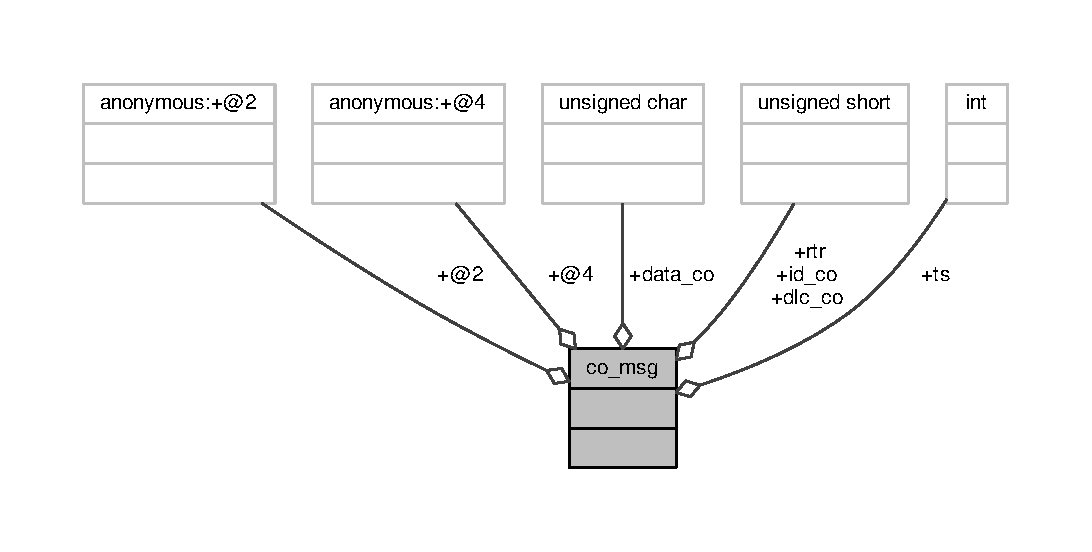
\includegraphics[width=350pt]{structco__msg__coll__graph}
\end{center}
\end{figure}
\subsection*{Public Attributes}
\begin{DoxyCompactItemize}
\item 
\begin{tabbing}
xx\=xx\=xx\=xx\=xx\=xx\=xx\=xx\=xx\=\kill
union \{\\
\>unsigned short \hyperlink{structco__msg_a634de83979d7da90565eccdf16304a07}{id\_co}\\
\}; \\

\end{tabbing}\item 
unsigned int \hyperlink{structco__msg_aaf8cd43d17baf495c982c87866fc90b2}{ts}
\item 
unsigned short \hyperlink{structco__msg_a4352880745fa6bc63d6c4e3c77870029}{rtr}\+:1
\item 
unsigned short \hyperlink{structco__msg_ab19d6996baf97d346427d9789d7e4a6b}{dlc\+\_\+co}
\item 
unsigned char \hyperlink{structco__msg_a3ced1bf4d72ca82fe53c829d42cd946e}{data\+\_\+co} \mbox{[}8\mbox{]}
\item 
\begin{tabbing}
xx\=xx\=xx\=xx\=xx\=xx\=xx\=xx\=xx\=\kill
union \{\\
\>unsigned short \hyperlink{structco__msg_a634de83979d7da90565eccdf16304a07}{id\_co}\\
\}; \\

\end{tabbing}\end{DoxyCompactItemize}


\subsection{Member Data Documentation}
\subsubsection[{\texorpdfstring{"@2}{@2}}]{\setlength{\rightskip}{0pt plus 5cm}union \{ ... \} }\hypertarget{structco__msg_af8251e2eaf9e807267d3ced55e292142}{}\label{structco__msg_af8251e2eaf9e807267d3ced55e292142}
\subsubsection[{\texorpdfstring{"@4}{@4}}]{\setlength{\rightskip}{0pt plus 5cm}union \{ ... \} }\hypertarget{structco__msg_a549464c55b7bbab6345f082dab73b275}{}\label{structco__msg_a549464c55b7bbab6345f082dab73b275}
\index{co\+\_\+msg@{co\+\_\+msg}!data\+\_\+co@{data\+\_\+co}}
\index{data\+\_\+co@{data\+\_\+co}!co\+\_\+msg@{co\+\_\+msg}}
\subsubsection[{\texorpdfstring{data\+\_\+co}{data_co}}]{\setlength{\rightskip}{0pt plus 5cm}unsigned char co\+\_\+msg\+::data\+\_\+co}\hypertarget{structco__msg_a3ced1bf4d72ca82fe53c829d42cd946e}{}\label{structco__msg_a3ced1bf4d72ca82fe53c829d42cd946e}
\index{co\+\_\+msg@{co\+\_\+msg}!dlc\+\_\+co@{dlc\+\_\+co}}
\index{dlc\+\_\+co@{dlc\+\_\+co}!co\+\_\+msg@{co\+\_\+msg}}
\subsubsection[{\texorpdfstring{dlc\+\_\+co}{dlc_co}}]{\setlength{\rightskip}{0pt plus 5cm}unsigned short co\+\_\+msg\+::dlc\+\_\+co}\hypertarget{structco__msg_ab19d6996baf97d346427d9789d7e4a6b}{}\label{structco__msg_ab19d6996baf97d346427d9789d7e4a6b}
\index{co\+\_\+msg@{co\+\_\+msg}!id\+\_\+co@{id\+\_\+co}}
\index{id\+\_\+co@{id\+\_\+co}!co\+\_\+msg@{co\+\_\+msg}}
\subsubsection[{\texorpdfstring{id\+\_\+co}{id_co}}]{\setlength{\rightskip}{0pt plus 5cm}unsigned short co\+\_\+msg\+::id\+\_\+co}\hypertarget{structco__msg_a634de83979d7da90565eccdf16304a07}{}\label{structco__msg_a634de83979d7da90565eccdf16304a07}
\index{co\+\_\+msg@{co\+\_\+msg}!rtr@{rtr}}
\index{rtr@{rtr}!co\+\_\+msg@{co\+\_\+msg}}
\subsubsection[{\texorpdfstring{rtr}{rtr}}]{\setlength{\rightskip}{0pt plus 5cm}unsigned short co\+\_\+msg\+::rtr}\hypertarget{structco__msg_a4352880745fa6bc63d6c4e3c77870029}{}\label{structco__msg_a4352880745fa6bc63d6c4e3c77870029}
\index{co\+\_\+msg@{co\+\_\+msg}!ts@{ts}}
\index{ts@{ts}!co\+\_\+msg@{co\+\_\+msg}}
\subsubsection[{\texorpdfstring{ts}{ts}}]{\setlength{\rightskip}{0pt plus 5cm}unsigned int co\+\_\+msg\+::ts}\hypertarget{structco__msg_aaf8cd43d17baf495c982c87866fc90b2}{}\label{structco__msg_aaf8cd43d17baf495c982c87866fc90b2}


The documentation for this struct was generated from the following files\+:\begin{DoxyCompactItemize}
\item 
\hyperlink{candatatypes_8h}{candatatypes.\+h}\item 
\hyperlink{co__msg_8h}{co\+\_\+msg.\+h}\end{DoxyCompactItemize}

\hypertarget{structerr__stat}{}\section{err\+\_\+stat Struct Reference}
\label{structerr__stat}\index{err\+\_\+stat@{err\+\_\+stat}}


{\ttfamily \#include $<$hico\+\_\+api.\+h$>$}



Collaboration diagram for err\+\_\+stat\+:\nopagebreak
\begin{figure}[H]
\begin{center}
\leavevmode
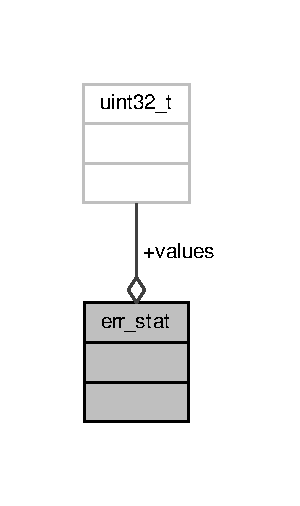
\includegraphics[width=144pt]{structerr__stat__coll__graph}
\end{center}
\end{figure}
\subsection*{Public Attributes}
\begin{DoxyCompactItemize}
\item 
uint32\+\_\+t \hyperlink{structerr__stat_a659e627af5963248da109c8e2404cd08}{values} \mbox{[}0x3f\mbox{]}
\end{DoxyCompactItemize}


\subsection{Member Data Documentation}
\index{err\+\_\+stat@{err\+\_\+stat}!values@{values}}
\index{values@{values}!err\+\_\+stat@{err\+\_\+stat}}
\subsubsection[{\texorpdfstring{values}{values}}]{\setlength{\rightskip}{0pt plus 5cm}uint32\+\_\+t err\+\_\+stat\+::values\mbox{[}0x3f\mbox{]}}\hypertarget{structerr__stat_a659e627af5963248da109c8e2404cd08}{}\label{structerr__stat_a659e627af5963248da109c8e2404cd08}


The documentation for this struct was generated from the following file\+:\begin{DoxyCompactItemize}
\item 
\hyperlink{hico__api_8h}{hico\+\_\+api.\+h}\end{DoxyCompactItemize}

\hypertarget{classPortBase}{}\section{Port\+Base Class Reference}
\label{classPortBase}\index{Port\+Base@{Port\+Base}}


{\ttfamily \#include $<$Port\+Base.\+h$>$}



Inheritance diagram for Port\+Base\+:
\nopagebreak
\begin{figure}[H]
\begin{center}
\leavevmode
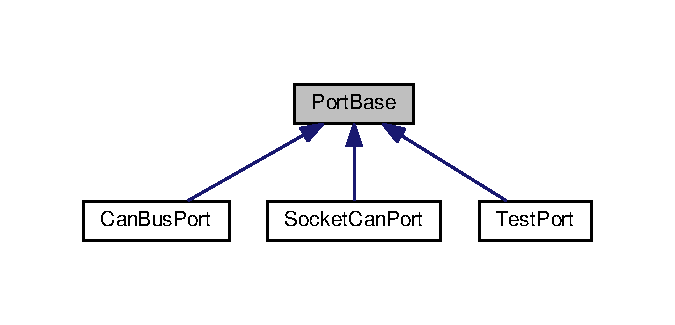
\includegraphics[width=350pt]{classPortBase__inherit__graph}
\end{center}
\end{figure}


Collaboration diagram for Port\+Base\+:
\nopagebreak
\begin{figure}[H]
\begin{center}
\leavevmode
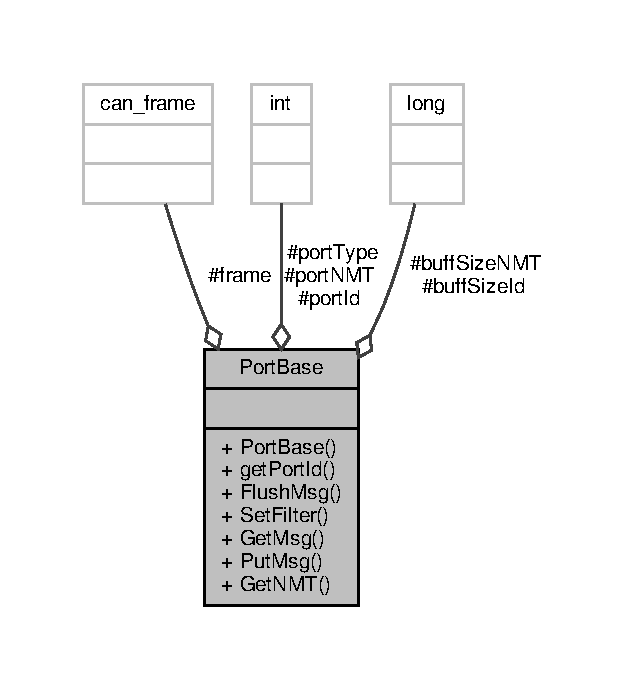
\includegraphics[width=301pt]{classPortBase__coll__graph}
\end{center}
\end{figure}
\subsection*{Public Member Functions}
\begin{DoxyCompactItemize}
\item 
\hyperlink{classPortBase_acb7872550bc94538ef95d2510d763be3}{Port\+Base} ()
\item 
int \hyperlink{classPortBase_a45ec4a2cd5e17e098f6f72677437f066}{get\+Port\+Id} ()
\item 
long \hyperlink{classPortBase_a913932fc850e9aebc947542773c669ad}{Flush\+Msg} ()
\item 
virtual long \hyperlink{classPortBase_a1d857a81a8e3f3bd460ef7c802ee762c}{Set\+Filter} (uint32\+\_\+t can\+Id, uint32\+\_\+t mask)=0
\item 
virtual long \hyperlink{classPortBase_a4fe82768f2b79889d7084292ac0e8696}{Get\+Msg} (uint32\+\_\+t \&can\+Id, uint8\+\_\+t $\ast$data, uint8\+\_\+t \&size)=0
\item 
virtual long \hyperlink{classPortBase_a26213ebb6ea0a0b77f60c28944e3bb8e}{Put\+Msg} (const uint32\+\_\+t \&can\+Id, uint8\+\_\+t $\ast$const data, const uint8\+\_\+t size)=0
\item 
virtual long \hyperlink{classPortBase_abab2bf17b01d87c2bca01cb2151aa2f1}{Get\+N\+MT} (uint8\+\_\+t $\ast$data, uint8\+\_\+t \&size)=0
\end{DoxyCompactItemize}
\subsection*{Protected Attributes}
\begin{DoxyCompactItemize}
\item 
int \hyperlink{classPortBase_af8816a6f73bf391d2948f3564f8ea1df}{port\+Id}
\item 
int \hyperlink{classPortBase_a6f18d480ef41a91fd2957927fe94c408}{port\+Type}
\item 
int \hyperlink{classPortBase_ae63f6df54bbeac1046b5dfbe178e1cee}{port\+N\+MT}
\item 
can\+\_\+frame \hyperlink{classPortBase_ae175156fa18f3be1820adea89ef7b13c}{frame}
\item 
long \hyperlink{classPortBase_a559431268076ea9b23bce545510f7b39}{buff\+Size\+Id}
\item 
long \hyperlink{classPortBase_aba8241e5d55c06c7d1a11ebb18096328}{buff\+Size\+N\+MT}
\end{DoxyCompactItemize}


\subsection{Constructor \& Destructor Documentation}
\index{Port\+Base@{Port\+Base}!Port\+Base@{Port\+Base}}
\index{Port\+Base@{Port\+Base}!Port\+Base@{Port\+Base}}
\subsubsection[{\texorpdfstring{Port\+Base()}{PortBase()}}]{\setlength{\rightskip}{0pt plus 5cm}Port\+Base\+::\+Port\+Base (
\begin{DoxyParamCaption}
{}
\end{DoxyParamCaption}
)}\hypertarget{classPortBase_acb7872550bc94538ef95d2510d763be3}{}\label{classPortBase_acb7872550bc94538ef95d2510d763be3}


\subsection{Member Function Documentation}
\index{Port\+Base@{Port\+Base}!Flush\+Msg@{Flush\+Msg}}
\index{Flush\+Msg@{Flush\+Msg}!Port\+Base@{Port\+Base}}
\subsubsection[{\texorpdfstring{Flush\+Msg()}{FlushMsg()}}]{\setlength{\rightskip}{0pt plus 5cm}long Port\+Base\+::\+Flush\+Msg (
\begin{DoxyParamCaption}
{}
\end{DoxyParamCaption}
)}\hypertarget{classPortBase_a913932fc850e9aebc947542773c669ad}{}\label{classPortBase_a913932fc850e9aebc947542773c669ad}
\index{Port\+Base@{Port\+Base}!Get\+Msg@{Get\+Msg}}
\index{Get\+Msg@{Get\+Msg}!Port\+Base@{Port\+Base}}
\subsubsection[{\texorpdfstring{Get\+Msg(uint32\+\_\+t \&can\+Id, uint8\+\_\+t $\ast$data, uint8\+\_\+t \&size)=0}{GetMsg(uint32_t &canId, uint8_t *data, uint8_t &size)=0}}]{\setlength{\rightskip}{0pt plus 5cm}virtual long Port\+Base\+::\+Get\+Msg (
\begin{DoxyParamCaption}
\item[{uint32\+\_\+t \&}]{can\+Id, }
\item[{uint8\+\_\+t $\ast$}]{data, }
\item[{uint8\+\_\+t \&}]{size}
\end{DoxyParamCaption}
)\hspace{0.3cm}{\ttfamily [pure virtual]}}\hypertarget{classPortBase_a4fe82768f2b79889d7084292ac0e8696}{}\label{classPortBase_a4fe82768f2b79889d7084292ac0e8696}


Implemented in \hyperlink{classCanBusPort_ac442e4e5b7bb154ea6322518b715f406}{Can\+Bus\+Port}, and \hyperlink{classSocketCanPort_aa9684efc602da057cb4928d52395af33}{Socket\+Can\+Port}.

\index{Port\+Base@{Port\+Base}!Get\+N\+MT@{Get\+N\+MT}}
\index{Get\+N\+MT@{Get\+N\+MT}!Port\+Base@{Port\+Base}}
\subsubsection[{\texorpdfstring{Get\+N\+M\+T(uint8\+\_\+t $\ast$data, uint8\+\_\+t \&size)=0}{GetNMT(uint8_t *data, uint8_t &size)=0}}]{\setlength{\rightskip}{0pt plus 5cm}virtual long Port\+Base\+::\+Get\+N\+MT (
\begin{DoxyParamCaption}
\item[{uint8\+\_\+t $\ast$}]{data, }
\item[{uint8\+\_\+t \&}]{size}
\end{DoxyParamCaption}
)\hspace{0.3cm}{\ttfamily [pure virtual]}}\hypertarget{classPortBase_abab2bf17b01d87c2bca01cb2151aa2f1}{}\label{classPortBase_abab2bf17b01d87c2bca01cb2151aa2f1}


Implemented in \hyperlink{classCanBusPort_a41242dc7980ca398e4770813e50ef32b}{Can\+Bus\+Port}, and \hyperlink{classSocketCanPort_a2efe27bd3bb8c8127c89925e1e21535a}{Socket\+Can\+Port}.

\index{Port\+Base@{Port\+Base}!get\+Port\+Id@{get\+Port\+Id}}
\index{get\+Port\+Id@{get\+Port\+Id}!Port\+Base@{Port\+Base}}
\subsubsection[{\texorpdfstring{get\+Port\+Id()}{getPortId()}}]{\setlength{\rightskip}{0pt plus 5cm}int Port\+Base\+::get\+Port\+Id (
\begin{DoxyParamCaption}
{}
\end{DoxyParamCaption}
)}\hypertarget{classPortBase_a45ec4a2cd5e17e098f6f72677437f066}{}\label{classPortBase_a45ec4a2cd5e17e098f6f72677437f066}
\index{Port\+Base@{Port\+Base}!Put\+Msg@{Put\+Msg}}
\index{Put\+Msg@{Put\+Msg}!Port\+Base@{Port\+Base}}
\subsubsection[{\texorpdfstring{Put\+Msg(const uint32\+\_\+t \&can\+Id, uint8\+\_\+t $\ast$const data, const uint8\+\_\+t size)=0}{PutMsg(const uint32_t &canId, uint8_t *const data, const uint8_t size)=0}}]{\setlength{\rightskip}{0pt plus 5cm}virtual long Port\+Base\+::\+Put\+Msg (
\begin{DoxyParamCaption}
\item[{const uint32\+\_\+t \&}]{can\+Id, }
\item[{uint8\+\_\+t $\ast$const}]{data, }
\item[{const uint8\+\_\+t}]{size}
\end{DoxyParamCaption}
)\hspace{0.3cm}{\ttfamily [pure virtual]}}\hypertarget{classPortBase_a26213ebb6ea0a0b77f60c28944e3bb8e}{}\label{classPortBase_a26213ebb6ea0a0b77f60c28944e3bb8e}


Implemented in \hyperlink{classCanBusPort_a2bb802ad7a14e260f0f51b79d4c53c43}{Can\+Bus\+Port}, and \hyperlink{classSocketCanPort_a9375a0c1e33978c83ebd188100898633}{Socket\+Can\+Port}.

\index{Port\+Base@{Port\+Base}!Set\+Filter@{Set\+Filter}}
\index{Set\+Filter@{Set\+Filter}!Port\+Base@{Port\+Base}}
\subsubsection[{\texorpdfstring{Set\+Filter(uint32\+\_\+t can\+Id, uint32\+\_\+t mask)=0}{SetFilter(uint32_t canId, uint32_t mask)=0}}]{\setlength{\rightskip}{0pt plus 5cm}virtual long Port\+Base\+::\+Set\+Filter (
\begin{DoxyParamCaption}
\item[{uint32\+\_\+t}]{can\+Id, }
\item[{uint32\+\_\+t}]{mask}
\end{DoxyParamCaption}
)\hspace{0.3cm}{\ttfamily [pure virtual]}}\hypertarget{classPortBase_a1d857a81a8e3f3bd460ef7c802ee762c}{}\label{classPortBase_a1d857a81a8e3f3bd460ef7c802ee762c}


Implemented in \hyperlink{classCanBusPort_af09c794e3af86e89c8a511535f856dc9}{Can\+Bus\+Port}, and \hyperlink{classSocketCanPort_a1a5d0866524dae11ddff0d1ac22e0dd5}{Socket\+Can\+Port}.



\subsection{Member Data Documentation}
\index{Port\+Base@{Port\+Base}!buff\+Size\+Id@{buff\+Size\+Id}}
\index{buff\+Size\+Id@{buff\+Size\+Id}!Port\+Base@{Port\+Base}}
\subsubsection[{\texorpdfstring{buff\+Size\+Id}{buffSizeId}}]{\setlength{\rightskip}{0pt plus 5cm}long Port\+Base\+::buff\+Size\+Id\hspace{0.3cm}{\ttfamily [protected]}}\hypertarget{classPortBase_a559431268076ea9b23bce545510f7b39}{}\label{classPortBase_a559431268076ea9b23bce545510f7b39}
\index{Port\+Base@{Port\+Base}!buff\+Size\+N\+MT@{buff\+Size\+N\+MT}}
\index{buff\+Size\+N\+MT@{buff\+Size\+N\+MT}!Port\+Base@{Port\+Base}}
\subsubsection[{\texorpdfstring{buff\+Size\+N\+MT}{buffSizeNMT}}]{\setlength{\rightskip}{0pt plus 5cm}long Port\+Base\+::buff\+Size\+N\+MT\hspace{0.3cm}{\ttfamily [protected]}}\hypertarget{classPortBase_aba8241e5d55c06c7d1a11ebb18096328}{}\label{classPortBase_aba8241e5d55c06c7d1a11ebb18096328}
\index{Port\+Base@{Port\+Base}!frame@{frame}}
\index{frame@{frame}!Port\+Base@{Port\+Base}}
\subsubsection[{\texorpdfstring{frame}{frame}}]{\setlength{\rightskip}{0pt plus 5cm}can\+\_\+frame Port\+Base\+::frame\hspace{0.3cm}{\ttfamily [protected]}}\hypertarget{classPortBase_ae175156fa18f3be1820adea89ef7b13c}{}\label{classPortBase_ae175156fa18f3be1820adea89ef7b13c}
\index{Port\+Base@{Port\+Base}!port\+Id@{port\+Id}}
\index{port\+Id@{port\+Id}!Port\+Base@{Port\+Base}}
\subsubsection[{\texorpdfstring{port\+Id}{portId}}]{\setlength{\rightskip}{0pt plus 5cm}int Port\+Base\+::port\+Id\hspace{0.3cm}{\ttfamily [protected]}}\hypertarget{classPortBase_af8816a6f73bf391d2948f3564f8ea1df}{}\label{classPortBase_af8816a6f73bf391d2948f3564f8ea1df}
\index{Port\+Base@{Port\+Base}!port\+N\+MT@{port\+N\+MT}}
\index{port\+N\+MT@{port\+N\+MT}!Port\+Base@{Port\+Base}}
\subsubsection[{\texorpdfstring{port\+N\+MT}{portNMT}}]{\setlength{\rightskip}{0pt plus 5cm}int Port\+Base\+::port\+N\+MT\hspace{0.3cm}{\ttfamily [protected]}}\hypertarget{classPortBase_ae63f6df54bbeac1046b5dfbe178e1cee}{}\label{classPortBase_ae63f6df54bbeac1046b5dfbe178e1cee}
\index{Port\+Base@{Port\+Base}!port\+Type@{port\+Type}}
\index{port\+Type@{port\+Type}!Port\+Base@{Port\+Base}}
\subsubsection[{\texorpdfstring{port\+Type}{portType}}]{\setlength{\rightskip}{0pt plus 5cm}int Port\+Base\+::port\+Type\hspace{0.3cm}{\ttfamily [protected]}}\hypertarget{classPortBase_a6f18d480ef41a91fd2957927fe94c408}{}\label{classPortBase_a6f18d480ef41a91fd2957927fe94c408}


The documentation for this class was generated from the following files\+:\begin{DoxyCompactItemize}
\item 
\hyperlink{PortBase_8h}{Port\+Base.\+h}\item 
\hyperlink{PortBase_8cpp}{Port\+Base.\+cpp}\end{DoxyCompactItemize}

\hypertarget{classSocketCanPort}{}\section{Socket\+Can\+Port Class Reference}
\label{classSocketCanPort}\index{Socket\+Can\+Port@{Socket\+Can\+Port}}


{\ttfamily \#include $<$Socket\+Can\+Port.\+h$>$}



Inheritance diagram for Socket\+Can\+Port\+:
\nopagebreak
\begin{figure}[H]
\begin{center}
\leavevmode
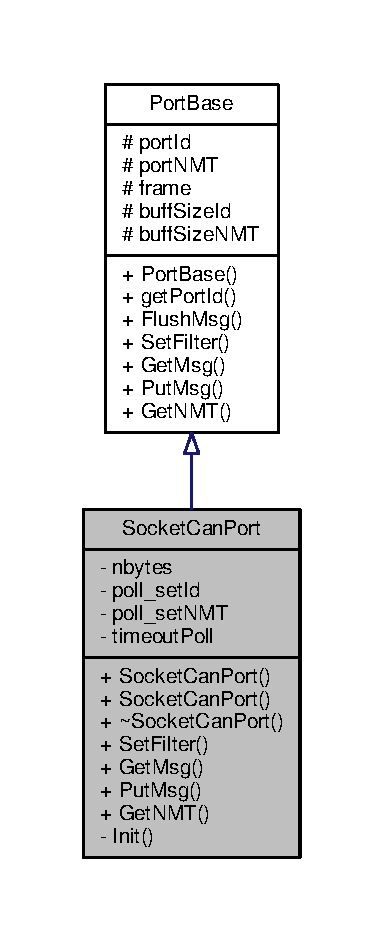
\includegraphics[width=184pt]{classSocketCanPort__inherit__graph}
\end{center}
\end{figure}


Collaboration diagram for Socket\+Can\+Port\+:
\nopagebreak
\begin{figure}[H]
\begin{center}
\leavevmode
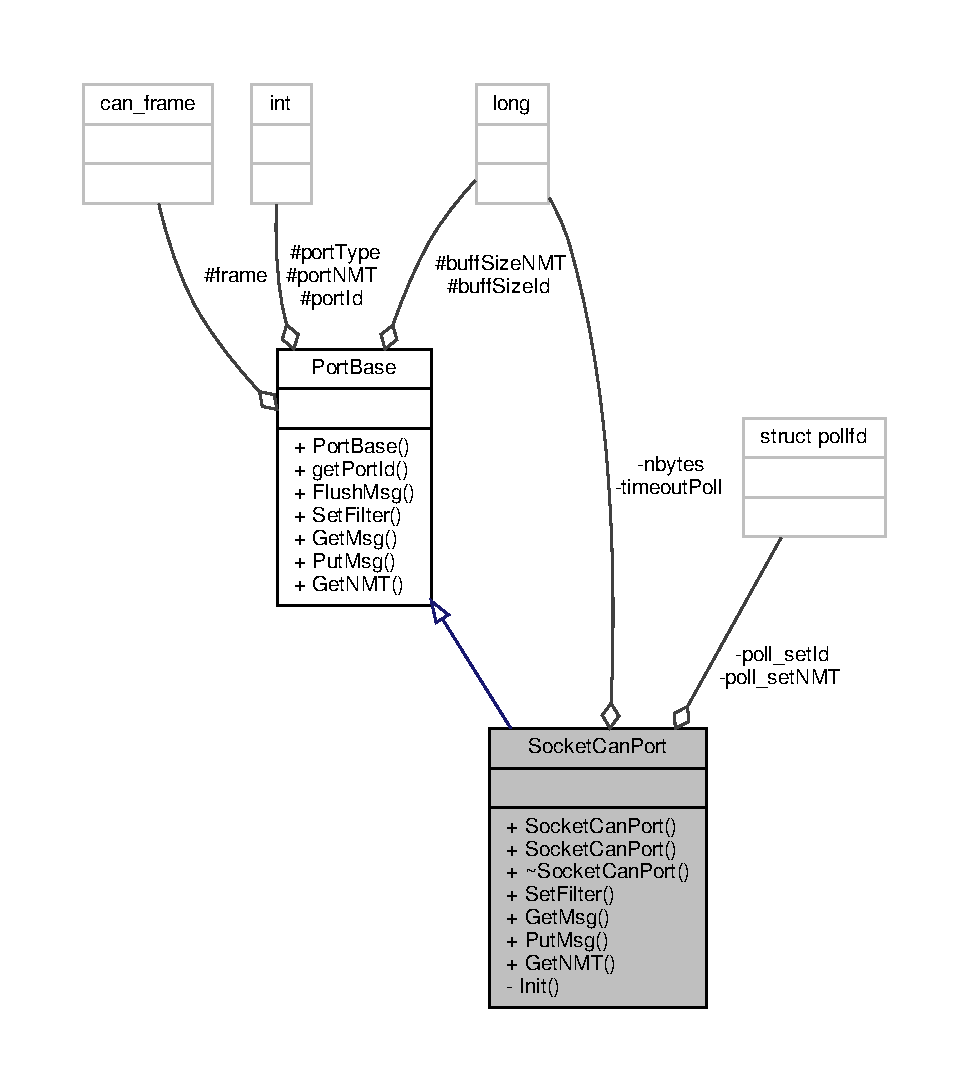
\includegraphics[width=350pt]{classSocketCanPort__coll__graph}
\end{center}
\end{figure}
\subsection*{Public Member Functions}
\begin{DoxyCompactItemize}
\item 
\hyperlink{classSocketCanPort_af3593609acea236b10646732e277837f}{Socket\+Can\+Port} ()
\item 
\hyperlink{classSocketCanPort_a087bc07f3c1658e3cb994d85fcb3da5e}{Socket\+Can\+Port} (string can\+Port)
\item 
\hyperlink{classSocketCanPort_a0d004347e49110daa1ee29e1d1bc85c0}{$\sim$\+Socket\+Can\+Port} ()
\item 
long \hyperlink{classSocketCanPort_a1a5d0866524dae11ddff0d1ac22e0dd5}{Set\+Filter} (uint32\+\_\+t can\+Id, uint32\+\_\+t mask)
\item 
long \hyperlink{classSocketCanPort_aa9684efc602da057cb4928d52395af33}{Get\+Msg} (uint32\+\_\+t \&can\+Id, uint8\+\_\+t $\ast$data, uint8\+\_\+t \&size)
\item 
long \hyperlink{classSocketCanPort_a9375a0c1e33978c83ebd188100898633}{Put\+Msg} (const uint32\+\_\+t \&can\+Id, uint8\+\_\+t $\ast$const data, const uint8\+\_\+t size)
\item 
long \hyperlink{classSocketCanPort_a2efe27bd3bb8c8127c89925e1e21535a}{Get\+N\+MT} (uint8\+\_\+t $\ast$data, uint8\+\_\+t \&size)
\end{DoxyCompactItemize}
\subsection*{Private Member Functions}
\begin{DoxyCompactItemize}
\item 
long \hyperlink{classSocketCanPort_a9209d295c98c12ab85ec61773b775bf4}{Init} (string can\+Port)
\end{DoxyCompactItemize}
\subsection*{Private Attributes}
\begin{DoxyCompactItemize}
\item 
long \hyperlink{classSocketCanPort_a7b06b4d8c897c1a189329f20632fdb71}{nbytes}
\item 
struct pollfd \hyperlink{classSocketCanPort_ad0374fe5ea78a061e7abd16b812f44d5}{poll\+\_\+set\+Id} \mbox{[}1\mbox{]}
\item 
struct pollfd \hyperlink{classSocketCanPort_afaaf9cd49684de93be7370988ec64b47}{poll\+\_\+set\+N\+MT} \mbox{[}1\mbox{]}
\item 
long \hyperlink{classSocketCanPort_a18e670bf7f98482e022da2fd11264309}{timeout\+Poll}
\end{DoxyCompactItemize}
\subsection*{Additional Inherited Members}


\subsection{Constructor \& Destructor Documentation}
\index{Socket\+Can\+Port@{Socket\+Can\+Port}!Socket\+Can\+Port@{Socket\+Can\+Port}}
\index{Socket\+Can\+Port@{Socket\+Can\+Port}!Socket\+Can\+Port@{Socket\+Can\+Port}}
\subsubsection[{\texorpdfstring{Socket\+Can\+Port()}{SocketCanPort()}}]{\setlength{\rightskip}{0pt plus 5cm}Socket\+Can\+Port\+::\+Socket\+Can\+Port (
\begin{DoxyParamCaption}
{}
\end{DoxyParamCaption}
)}\hypertarget{classSocketCanPort_af3593609acea236b10646732e277837f}{}\label{classSocketCanPort_af3593609acea236b10646732e277837f}
\index{Socket\+Can\+Port@{Socket\+Can\+Port}!Socket\+Can\+Port@{Socket\+Can\+Port}}
\index{Socket\+Can\+Port@{Socket\+Can\+Port}!Socket\+Can\+Port@{Socket\+Can\+Port}}
\subsubsection[{\texorpdfstring{Socket\+Can\+Port(string can\+Port)}{SocketCanPort(string canPort)}}]{\setlength{\rightskip}{0pt plus 5cm}Socket\+Can\+Port\+::\+Socket\+Can\+Port (
\begin{DoxyParamCaption}
\item[{string}]{can\+Port}
\end{DoxyParamCaption}
)}\hypertarget{classSocketCanPort_a087bc07f3c1658e3cb994d85fcb3da5e}{}\label{classSocketCanPort_a087bc07f3c1658e3cb994d85fcb3da5e}
\index{Socket\+Can\+Port@{Socket\+Can\+Port}!````~Socket\+Can\+Port@{$\sim$\+Socket\+Can\+Port}}
\index{````~Socket\+Can\+Port@{$\sim$\+Socket\+Can\+Port}!Socket\+Can\+Port@{Socket\+Can\+Port}}
\subsubsection[{\texorpdfstring{$\sim$\+Socket\+Can\+Port()}{~SocketCanPort()}}]{\setlength{\rightskip}{0pt plus 5cm}Socket\+Can\+Port\+::$\sim$\+Socket\+Can\+Port (
\begin{DoxyParamCaption}
{}
\end{DoxyParamCaption}
)}\hypertarget{classSocketCanPort_a0d004347e49110daa1ee29e1d1bc85c0}{}\label{classSocketCanPort_a0d004347e49110daa1ee29e1d1bc85c0}


\subsection{Member Function Documentation}
\index{Socket\+Can\+Port@{Socket\+Can\+Port}!Get\+Msg@{Get\+Msg}}
\index{Get\+Msg@{Get\+Msg}!Socket\+Can\+Port@{Socket\+Can\+Port}}
\subsubsection[{\texorpdfstring{Get\+Msg(uint32\+\_\+t \&can\+Id, uint8\+\_\+t $\ast$data, uint8\+\_\+t \&size)}{GetMsg(uint32_t &canId, uint8_t *data, uint8_t &size)}}]{\setlength{\rightskip}{0pt plus 5cm}long Socket\+Can\+Port\+::\+Get\+Msg (
\begin{DoxyParamCaption}
\item[{uint32\+\_\+t \&}]{can\+Id, }
\item[{uint8\+\_\+t $\ast$}]{data, }
\item[{uint8\+\_\+t \&}]{size}
\end{DoxyParamCaption}
)\hspace{0.3cm}{\ttfamily [virtual]}}\hypertarget{classSocketCanPort_aa9684efc602da057cb4928d52395af33}{}\label{classSocketCanPort_aa9684efc602da057cb4928d52395af33}


Implements \hyperlink{classPortBase_a4fe82768f2b79889d7084292ac0e8696}{Port\+Base}.

\index{Socket\+Can\+Port@{Socket\+Can\+Port}!Get\+N\+MT@{Get\+N\+MT}}
\index{Get\+N\+MT@{Get\+N\+MT}!Socket\+Can\+Port@{Socket\+Can\+Port}}
\subsubsection[{\texorpdfstring{Get\+N\+M\+T(uint8\+\_\+t $\ast$data, uint8\+\_\+t \&size)}{GetNMT(uint8_t *data, uint8_t &size)}}]{\setlength{\rightskip}{0pt plus 5cm}long Socket\+Can\+Port\+::\+Get\+N\+MT (
\begin{DoxyParamCaption}
\item[{uint8\+\_\+t $\ast$}]{data, }
\item[{uint8\+\_\+t \&}]{size}
\end{DoxyParamCaption}
)\hspace{0.3cm}{\ttfamily [virtual]}}\hypertarget{classSocketCanPort_a2efe27bd3bb8c8127c89925e1e21535a}{}\label{classSocketCanPort_a2efe27bd3bb8c8127c89925e1e21535a}


Implements \hyperlink{classPortBase_abab2bf17b01d87c2bca01cb2151aa2f1}{Port\+Base}.

\index{Socket\+Can\+Port@{Socket\+Can\+Port}!Init@{Init}}
\index{Init@{Init}!Socket\+Can\+Port@{Socket\+Can\+Port}}
\subsubsection[{\texorpdfstring{Init(string can\+Port)}{Init(string canPort)}}]{\setlength{\rightskip}{0pt plus 5cm}long Socket\+Can\+Port\+::\+Init (
\begin{DoxyParamCaption}
\item[{string}]{can\+Port}
\end{DoxyParamCaption}
)\hspace{0.3cm}{\ttfamily [private]}}\hypertarget{classSocketCanPort_a9209d295c98c12ab85ec61773b775bf4}{}\label{classSocketCanPort_a9209d295c98c12ab85ec61773b775bf4}
\index{Socket\+Can\+Port@{Socket\+Can\+Port}!Put\+Msg@{Put\+Msg}}
\index{Put\+Msg@{Put\+Msg}!Socket\+Can\+Port@{Socket\+Can\+Port}}
\subsubsection[{\texorpdfstring{Put\+Msg(const uint32\+\_\+t \&can\+Id, uint8\+\_\+t $\ast$const data, const uint8\+\_\+t size)}{PutMsg(const uint32_t &canId, uint8_t *const data, const uint8_t size)}}]{\setlength{\rightskip}{0pt plus 5cm}long Socket\+Can\+Port\+::\+Put\+Msg (
\begin{DoxyParamCaption}
\item[{const uint32\+\_\+t \&}]{can\+Id, }
\item[{uint8\+\_\+t $\ast$const}]{data, }
\item[{const uint8\+\_\+t}]{size}
\end{DoxyParamCaption}
)\hspace{0.3cm}{\ttfamily [virtual]}}\hypertarget{classSocketCanPort_a9375a0c1e33978c83ebd188100898633}{}\label{classSocketCanPort_a9375a0c1e33978c83ebd188100898633}


Implements \hyperlink{classPortBase_a26213ebb6ea0a0b77f60c28944e3bb8e}{Port\+Base}.

\index{Socket\+Can\+Port@{Socket\+Can\+Port}!Set\+Filter@{Set\+Filter}}
\index{Set\+Filter@{Set\+Filter}!Socket\+Can\+Port@{Socket\+Can\+Port}}
\subsubsection[{\texorpdfstring{Set\+Filter(uint32\+\_\+t can\+Id, uint32\+\_\+t mask)}{SetFilter(uint32_t canId, uint32_t mask)}}]{\setlength{\rightskip}{0pt plus 5cm}long Socket\+Can\+Port\+::\+Set\+Filter (
\begin{DoxyParamCaption}
\item[{uint32\+\_\+t}]{can\+Id, }
\item[{uint32\+\_\+t}]{mask}
\end{DoxyParamCaption}
)\hspace{0.3cm}{\ttfamily [virtual]}}\hypertarget{classSocketCanPort_a1a5d0866524dae11ddff0d1ac22e0dd5}{}\label{classSocketCanPort_a1a5d0866524dae11ddff0d1ac22e0dd5}


Implements \hyperlink{classPortBase_a1d857a81a8e3f3bd460ef7c802ee762c}{Port\+Base}.



\subsection{Member Data Documentation}
\index{Socket\+Can\+Port@{Socket\+Can\+Port}!nbytes@{nbytes}}
\index{nbytes@{nbytes}!Socket\+Can\+Port@{Socket\+Can\+Port}}
\subsubsection[{\texorpdfstring{nbytes}{nbytes}}]{\setlength{\rightskip}{0pt plus 5cm}long Socket\+Can\+Port\+::nbytes\hspace{0.3cm}{\ttfamily [private]}}\hypertarget{classSocketCanPort_a7b06b4d8c897c1a189329f20632fdb71}{}\label{classSocketCanPort_a7b06b4d8c897c1a189329f20632fdb71}
\index{Socket\+Can\+Port@{Socket\+Can\+Port}!poll\+\_\+set\+Id@{poll\+\_\+set\+Id}}
\index{poll\+\_\+set\+Id@{poll\+\_\+set\+Id}!Socket\+Can\+Port@{Socket\+Can\+Port}}
\subsubsection[{\texorpdfstring{poll\+\_\+set\+Id}{poll_setId}}]{\setlength{\rightskip}{0pt plus 5cm}struct pollfd Socket\+Can\+Port\+::poll\+\_\+set\+Id\mbox{[}1\mbox{]}\hspace{0.3cm}{\ttfamily [private]}}\hypertarget{classSocketCanPort_ad0374fe5ea78a061e7abd16b812f44d5}{}\label{classSocketCanPort_ad0374fe5ea78a061e7abd16b812f44d5}
\index{Socket\+Can\+Port@{Socket\+Can\+Port}!poll\+\_\+set\+N\+MT@{poll\+\_\+set\+N\+MT}}
\index{poll\+\_\+set\+N\+MT@{poll\+\_\+set\+N\+MT}!Socket\+Can\+Port@{Socket\+Can\+Port}}
\subsubsection[{\texorpdfstring{poll\+\_\+set\+N\+MT}{poll_setNMT}}]{\setlength{\rightskip}{0pt plus 5cm}struct pollfd Socket\+Can\+Port\+::poll\+\_\+set\+N\+MT\mbox{[}1\mbox{]}\hspace{0.3cm}{\ttfamily [private]}}\hypertarget{classSocketCanPort_afaaf9cd49684de93be7370988ec64b47}{}\label{classSocketCanPort_afaaf9cd49684de93be7370988ec64b47}
\index{Socket\+Can\+Port@{Socket\+Can\+Port}!timeout\+Poll@{timeout\+Poll}}
\index{timeout\+Poll@{timeout\+Poll}!Socket\+Can\+Port@{Socket\+Can\+Port}}
\subsubsection[{\texorpdfstring{timeout\+Poll}{timeoutPoll}}]{\setlength{\rightskip}{0pt plus 5cm}long Socket\+Can\+Port\+::timeout\+Poll\hspace{0.3cm}{\ttfamily [private]}}\hypertarget{classSocketCanPort_a18e670bf7f98482e022da2fd11264309}{}\label{classSocketCanPort_a18e670bf7f98482e022da2fd11264309}


The documentation for this class was generated from the following files\+:\begin{DoxyCompactItemize}
\item 
\hyperlink{SocketCanPort_8h}{Socket\+Can\+Port.\+h}\item 
\hyperlink{SocketCanPort_8cpp}{Socket\+Can\+Port.\+cpp}\end{DoxyCompactItemize}

\hypertarget{classTestPort}{}\section{Test\+Port Class Reference}
\label{classTestPort}\index{Test\+Port@{Test\+Port}}


Inheritance diagram for Test\+Port\+:
\nopagebreak
\begin{figure}[H]
\begin{center}
\leavevmode
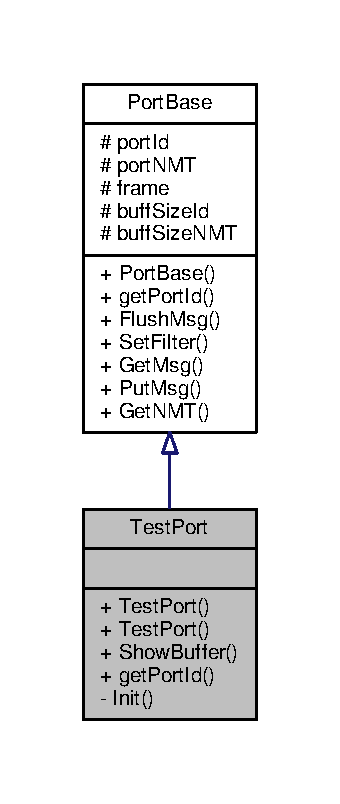
\includegraphics[width=137pt]{classTestPort__inherit__graph}
\end{center}
\end{figure}


Collaboration diagram for Test\+Port\+:
\nopagebreak
\begin{figure}[H]
\begin{center}
\leavevmode
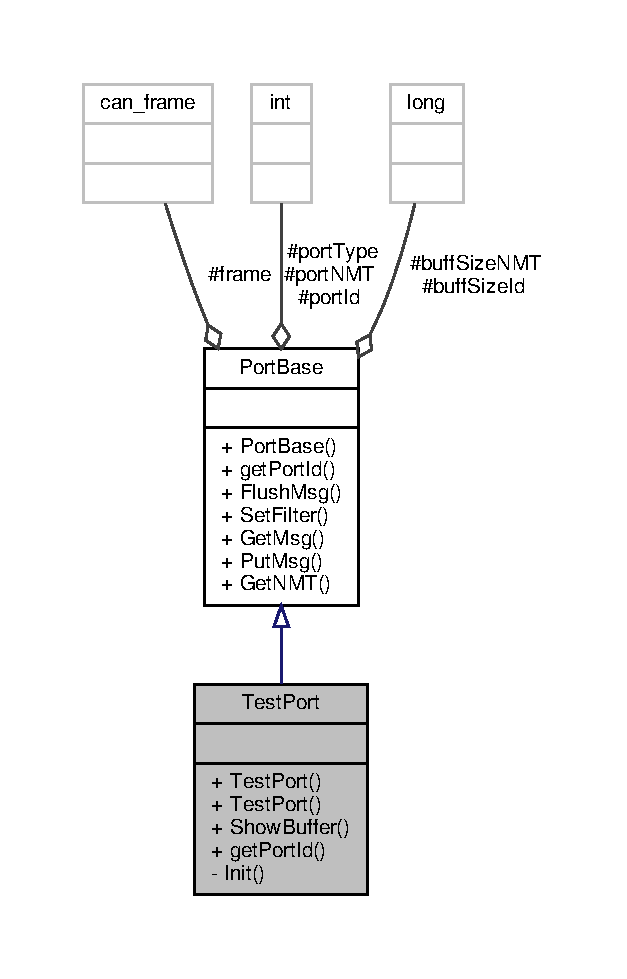
\includegraphics[width=137pt]{classTestPort__coll__graph}
\end{center}
\end{figure}
\subsection*{Public Member Functions}
\begin{DoxyCompactItemize}
\item 
\mbox{\Hypertarget{classTestPort_a93293d14818c76db0b4ef1273cf5ce19}\label{classTestPort_a93293d14818c76db0b4ef1273cf5ce19}} 
{\bfseries Test\+Port} (string Port)
\item 
\mbox{\Hypertarget{classTestPort_acc9bf1db6c1ca7d9040591306100ab36}\label{classTestPort_acc9bf1db6c1ca7d9040591306100ab36}} 
long {\bfseries Show\+Buffer} ()
\item 
\mbox{\Hypertarget{classTestPort_abf6a7327e26838aaf3e2e4482668085f}\label{classTestPort_abf6a7327e26838aaf3e2e4482668085f}} 
int {\bfseries get\+Port\+Id} ()
\end{DoxyCompactItemize}
\subsection*{Additional Inherited Members}


The documentation for this class was generated from the following files\+:\begin{DoxyCompactItemize}
\item 
Test\+Port.\+h\item 
Test\+Port.\+cpp\end{DoxyCompactItemize}

%--- End generated contents ---

% Index
\backmatter
\newpage
\phantomsection
\clearemptydoublepage
\addcontentsline{toc}{chapter}{Index}
\printindex

\end{document}
